\documentclass[10pt,a4paper]{article}
\usepackage[margin=1in]{geometry}
\usepackage[T1]{fontenc}
\usepackage[utf8]{inputenc}
\usepackage{amsmath,amssymb}
\usepackage{booktabs}
\usepackage{graphicx}
\usepackage{url}
\graphicspath{{figures/}}
\setlength{\parskip}{4pt}
\emergencystretch=2em

\title{Frozen Probes versus Matched Budgets: Protocol-Dependent Ordering of CLIP and ResNet-18 for Fine-Grained Tobacco Leaf-Disorder Classification}
\author{
Chenfeng Long$^{1,2,3}$, Zhiyong Tan$^{1,2,3}$, Yangjun Deng$^{1,2,3}$,\\ Xiang Luo$^{4}$, and Lizhuo Zhang$^{1,2,3*}$\\[6pt]
$^{1}$College of Information and Intelligence,\\
\hspace{1em}Hunan Agricultural University, Changsha 410128, China\\
$^{2}$Yuelushan Laboratory, Changsha 410128, China\\
$^{3}$Hunan Provincial Engineering and Technology Research\\
\hspace{1em}Center for Rural and Agricultural Informatization,\\
\hspace{1em}Hunan Agricultural University, Changsha 410128, China\\
$^{4}$Information Department, China Guangdong Tobacco\\
\hspace{1em}Meizhou Ltd, Meizhou 514000, China\\[4pt]
$^{*}$Corresponding author: L.~Zhang (zhanglizhuo@hunau.edu.cn)\\[4pt]
\parbox{\dimexpr\hsize-2\tabcolsep\relax}{\sloppy\small\textbf{Funding:} This work was supported in part by the Yuelushan Laboratory Breeding Program under Grant YLS-2026-ZY01002, in part by the National Natural Science Foundation of China (Youth Program) under Grant 62401203, and in part by the Meizhou Tobacco Science Research Project under Grant 202404.}
}
\date{}

\begin{document}
\maketitle

\begin{abstract}
Whether frozen CLIP probes can rival fine-tuned compact CNNs depends critically on the adaptation budget: with matched fine-tuning budgets, fine-tuned CLIP leads matched-budget ResNet-18 at every measured few-shot $K$ (with a smaller, non-significant full-data gap for DFN-CLIP, $p{=}0.12$), while at the default probe $C{=}1$ the apparent few-shot CLIP advantage over the legacy baseline was an artifact of the under-tuned CNN and is not present once the CNN receives a matched tuning budget; the probe side is likewise budget-sensitive, with validation-selected $C$ reversing the $K{=}1/2$ ordering for LAION-2B. We compared two generic CLIP checkpoints (DFN-CLIP, LAION-2B; ViT-L/14, 428M parameters) against a fine-tuned ResNet-18 (12M) on \emph{tobacco} leaf disorders (TPDD, 16 classes) in the zero-shot, few-shot ($K\in\{1,5,10\}$) and full-data regimes, with cross-crop checks on tomato and corn (both PlantVillage).
Under matched fine-tuning, fine-tuned CLIP leads matched ResNet-18 at every measured $K$ for both checkpoints (e.g., $85.1\%$ vs.\ $74.6\%$ at $K{=}10$ for DFN-CLIP), with all eight fine-tuning contrasts surviving Holm--Bonferroni correction. In the frozen-probe regime (at the default $C{=}1$), ResNet-18 leads or ties both CLIP probes at every measured $K$ when given a matched tuning budget (at $K{=}1$: 40.4\% vs.\ LAION-2B 40.1\% and DFN-CLIP 30.5\%; at $K{=}2$: 52.5\% vs.\ 48.8\% and 36.5\%; a $C$-grid sweep with validation-selected $C$ (single-seed) shows the probe side is likewise budget-sensitive: LAION-2B leads at $K{=}1$ (46.4\% vs.\ 40.4\%) and $K{=}2$ (55.1\% vs.\ 52.5\%), while DFN-CLIP still trails). The apparent $K{=}1$ LAION-2B lead over the legacy single-configuration baseline (40.1\% vs.\ 33.0\%) disappears once the baseline receives the same tuning budget. At full data, 5-fold cross-validation gave fine-tuned ResNet-18 a small, sign-stable edge over the validation-regularized frozen CLIP probe ($92.5\%$ vs.\ $89.4\%$); fine-tuned CLIP is numerically ahead for both checkpoints (LAION-2B $94.8\%$ vs.\ $92.5\%$, fold-level $p{=}0.03$, 5/5 folds; DFN-CLIP $93.7\%$ vs.\ $92.5\%$, fold-level $p{=}0.12$, 4/5 folds; these fold-level tests are descriptive and not part of the 16-contrast Holm family).
Zero-shot classification failed for every frozen image--text encoder we test: the best of 14 prompt templates sits at or below the 13.0\% majority-class baseline ($11.6\%$, $12.3\%$, $10.1\%$, $13.0\%$ for DFN-CLIP, LAION-2B, BioCLIP~2, and SigLIP; none significantly above it; one-sided exact binomial $p{=}0.73$/$0.64$/$0.87$/$0.54$ for DFN-CLIP/LAION-2B/BioCLIP~2/SigLIP, respectively; all $p>0.05$). The frozen features are not the limiting factor---they reach 86.2\% under a supervised probe---so the failure reflects a mismatch between the zero-shot text--image decision rule and the visual signal.
The cross-crop check reproduces the protocol-dependent pattern: fine-tuned ResNet-18 leads the frozen CLIP probe at $K{\geq}5$ on both crops, and the $K{=}1$ contrast is a tie within noise on both (tomato 44.7\% vs.\ 45.5\%; corn 76.8\% vs.\ 76.2\%); the two crops are reported separately rather than pooled, because PlantVillage's shared collection pipeline makes their errors non-independent and they should not be treated as independent evidence.
Readout geometry was checkpoint-dependent: on LAION-2B the patch tokens carry additional signal the CLS readout misses (mean-pool $+10.9$\,pp at $C{=}1$; though CLS at $C{=}100$ reaches 87.7\%, so the gain is $C$-dependent, not unconditional).
A field-condition evaluation (246 images, 19 classes) shows the fine-tuned ranking reverses under field conditions (ResNet-18 leads CLIP by 6.9\,pp), consistent with, but not attributable to, an image-style effect.
Practically: zero-shot CLIP should not be deployed for this task; the frozen and fine-tuned arms should be chosen by the binding constraint---iteration cost and reproducibility, accuracy, or inference cost. All code, data, and scripts are available in the repository cited in the Data Availability Statement.
\end{abstract}

\noindent\textbf{Keywords:} CLIP; zero-shot classification; agricultural disease diagnosis; vision-language models; few-shot learning; knowledge graph; prompt engineering



%%%%%%%%%%%%%%%%%%%%%%%%%%%%%%%%%%%%%%%%%%
\section{Introduction}
\label{sec:intro}

Vision-language models (VLMs) pretrained on web-scale image-text pairs, such as CLIP~\cite{radford2021learning}, have achieved strong zero-shot generalization across general-purpose visual recognition benchmarks.
This has led to growing enthusiasm for applying VLMs to specialized domains---including agriculture~\cite{pdclip2026}, medicine~\cite{huang2021gloria}, and remote sensing~\cite{liu2024remoteclip}---under the implicit assumption that large-scale pretraining transfers without additional training.

However, the visual statistics of specialized domains differ fundamentally from general web images.
Agricultural disease images feature fine-grained, domain-specific patterns (e.g., leaf lesions, fungal mycelia, chlorosis) that may be underrepresented in web-scale training corpora.
Whether and to what extent generic VLMs recognize these patterns remains an open empirical question with significant practical implications: if VLMs fail, practitioners would be misled; if they succeed, annotation costs could be reduced.

Recent work has explored domain-specific VLM adaptations. SCOLD~\cite{scold2025} pretrains a vision-language foundation model on over 186,000 leaf image-caption pairs, while BioCLIP 2~\cite{bioclip2} shows that 214M organism-image contrastive pretraining yields emergent zero-shot abilities on biological tasks. LP++~\cite{lpplus} proposes a learnable image-text knowledge blending linear probe that significantly surpasses naive CLIP probing. These adaptations require large-scale domain-specific pretraining; we empirically evaluate one such model, BioCLIP 2, as a domain-VLM control in the zero-shot results below and find it likewise sits below the majority-class baseline (10.1\% vs.\ 13.0\%).

In contrast, off-the-shelf CLIP is evaluated without agricultural fine-tuning---a question of immediate relevance for practitioners lacking resources for domain-specific pretraining. This work provides an empirical boundary for off-the-shelf CLIP's applicability in resource-constrained settings, systematically comparing against ResNet-18 across data regimes and testing whether KG-augmented prompts can mitigate the lack of domain adaptation. Our core contribution is a within-crop boundary for off-the-shelf CLIP on tobacco; to test whether the regime-by-regime pattern is crop-specific or more general, we additionally replicate the full protocol on two further crops (tomato and corn, both PlantVillage) under the identical split, probe, and evaluation conditions.

This investigation is guided by three research questions:

\begin{itemize}
    \item \textbf{RQ1.} Can CLIP zero-shot classify tobacco diseases, and do KG-augmented prompts help?
    \item \textbf{RQ2.} How does CLIP linear probe compare to end-to-end ResNet-18 across data regimes?
    \item \textbf{RQ3.} Do the zero-shot / few-shot / full-data model rankings generalize across crops (tomato PlantVillage in addition to tobacco TPDD and TLD)?
\end{itemize}

Five main findings are reported:
(1) Under matched fine-tuning budgets, fine-tuned CLIP leads fine-tuned ResNet-18 at every measured $K$ for both checkpoints (e.g., $85.1\%$ vs.\ $74.6\%$ at $K{=}10$ for DFN-CLIP; $79.3\%$ vs.\ $74.6\%$ for LAION-2B), with all eight seed-paired contrasts surviving Holm--Bonferroni correction ($15/16$ of the full $16$-contrast family significant after Holm--Bonferroni; individual contrast $p$-values: \texttt{data/multiplicity\_16\_matched\_corrected.json}). The frozen-probe ordering, a common assumption, is not a fixed property of the representations; it depends on both the CNN's tuning budget and the probe's regularization: at the default probe $C{=}1$, the apparent few-shot CLIP advantage over the legacy baseline was an artifact of the under-tuned CNN and is not present once the CNN receives a matched tuning budget (at $K{=}1$: 40.1\% LAION-2B vs.\ 40.4\% ResNet-18, a tie within noise; at $K{=}2$: 48.8\% vs.\ 52.5\%, ResNet-18 leads); the probe side is likewise budget-sensitive---with validation-selected $C$ (single-seed estimate; Methods), LAION-2B leads at $K{=}1$ (46.4\% vs.\ 40.4\%) and $K{=}2$ (55.1\% vs.\ 52.5\%), while DFN-CLIP still trails. At full data the primary evidence is 5-fold cross-validation, where ResNet-18 leads the validation-regularized probe by a small, sign-stable margin ($92.5\%$ vs.\ $89.4\%$); the 138-image held-out split (86.2\% vs.\ 87.7\%) cannot resolve that difference. Per-regime effect sizes, confidence intervals and multiplicity are in Section~\ref{sec:results}.
(2) Zero-shot classification shows no detectable improvement over the majority-class baseline for fine-grained tobacco lesions: for every frozen image--text model we test (two generic CLIP variants, the domain-specific BioCLIP~2, and SigLIP), the best of 14 prompt templates sits at or below the 13.0\% always-predict-the-common-class baseline ($11.6\%$, $12.3\%$, $10.1\%$, $13.0\%$ respectively), and KG-augmented prompts give no reliable gain over plain captions. The frozen features are not the limiting factor---they reach 86.2\% under a supervised probe---so the failure reflects a mismatch between the zero-shot text--image decision rule and the visual signal, not poor visual separability (inter/intra-class ratio 0.62 on the training split, 0.81 on the held-out split). The at-or-below-baseline zero-shot failure also holds on the external TLD set (best 6.9\% for DFN-CLIP vs.\ a 19.0\% majority baseline).
(3) The cross-crop check (tomato, 18{,}160 images, and corn, 3{,}852 images, both PlantVillage) reproduces the protocol-dependent ordering on test sets with adequate power (1{,}635 and 346 held-out images): fine-tuned ResNet-18 leads the frozen CLIP probe at $K{\geq}5$, significantly on both crops at $K{=}5$ and $K{=}10$. Against the matched-budget ResNet baseline (9-config validation-selected search, $n{=}15$), the $K{=}1$ contrast is a tie within noise on both crops: tomato 44.7\% vs.\ 45.5\% ($-0.8$\,pp) and corn 76.8\% vs.\ 76.2\% ($+0.6$\,pp)---consistent with the TPDD finding that the frozen-probe comparison is baseline-tuning-dependent. At full data both models saturate at 98--99.7\%, so that regime supports the ordering and sign of the tobacco result, not its near-ceiling magnitudes.
(4) Readout geometry is checkpoint-dependent: on LAION-2B the patch tokens carry additional signal the CLS readout misses (mean-pool $+10.9$\,pp at $C{=}1$; though CLS at $C{=}100$ reaches 87.7\%, so the gain is $C$-dependent). On DFN-CLIP the CLS token already carries essentially all signal. Directionally consistent with~\cite{shi2026registers}; reported as a characterization, not a new method.
(5) A directional field-condition check (53 test images, 19 classes; underpowered) suggests the fine-tuned ranking may reverse (ResNet-18 leads CLIP by 6.9\,pp), consistent with, but not attributable to, an image-style effect.

%%%%%%%%%%%%%%%%%%%%%%%%%%%%%%%%%%%%%%%%%%
\section{Related Work}
\label{sec:related}

\subsection{Vision-Language Models for Specialized Domains}

CLIP~\cite{radford2021learning} and its variants~\cite{zhai2023sigmoid,cherti2023reproducible} have enabled zero-shot image classification through natural language prompts, achieving strong results on standard benchmarks such as ImageNet~\cite{deng2009imagenet}, but systematic evaluation on small, imbalanced agricultural datasets remains limited.
Subsequent work has explored domain-specific adaptations such as BioCLIP~\cite{stevens2024bioclip} for organism classification and medical VLMs for radiology~\cite{huang2021gloria}, alongside agriculture-specific evaluation via the AgroBench vision-language benchmark~\cite{shinoda2025agrobench}.
In the leaf-disease domain specifically, SCOLD~\cite{scold2025} pretrains a vision-language foundation model on over 186,000 leaf image-caption pairs, and BioCLIP 2~\cite{bioclip2} shows that 214M organism-image contrastive pretraining yields emergent zero-shot abilities on biological tasks.
These adaptations require large-scale domain-specific pretraining.
In contrast, off-the-shelf CLIP is evaluated without agricultural fine-tuning---a question of immediate relevance for practitioners lacking resources for domain-specific pretraining.

\subsection{CLIP Prompt Engineering}

Prompt design significantly affects CLIP zero-shot performance~\cite{zhou2022learning,liu2025finegrained}, and domain-specific prompts have been reported to outperform generic ones in specialized settings.
Prior work has proposed prompt ensembling~\cite{radford2021learning}, learnable contexts~\cite{zhou2022learning}, and class-specific templates.
In agricultural domains, KGs encode structured disease information~\cite{cropdpkg2025}.
It is tested whether KG-derived symptom descriptions, a text-only pathway for injecting domain knowledge, can improve CLIP zero-shot classification.

\subsection{Few-Shot vs.\ Zero-Shot in Agriculture}

Few-shot learning has been studied for crop disease classification~\cite{argueso2020fewshot,liang2021cotton}, building on the large PlantVillage dataset~\cite{plantvillage2016} that established the standard benchmark for leaf-disease classification.
Systematic comparisons between zero-shot VLMs and few-shot domain models remain rare.
Agriculture-specific vision-language benchmarks such as AgroBench~\cite{shinoda2025agrobench} evaluate existing models on crop tasks but do not, in the surveyed literature, report controlled multi-seed replication of zero-shot results.
This work provides a statistically rigorous head-to-head comparison across two datasets.

%%%%%%%%%%%%%%%%%%%%%%%%%%%%%%%%%%%%%%%%%%
\section{Materials and Methods}
\label{sec:method}

\subsection{Datasets}

TPDD~\cite{lin2022tpdd} (our re-derived release copy presents a 16-class taxonomy with 1,571 images, following the companion TLA taxonomy~\cite{lin2024tla}---the SPIE record itself documents 2,721 field images with a 12-class identification subset, so the citation identifies the dataset lineage rather than the image census used here; a stratified $\approx$82/9/9 train/val/test split with exact counts 1,295/138/138; one image removed from the original 1,572 release due to corruption) is used as the primary dataset, and TLD~\cite{tld} (1,392 images, 10 classes) for cross-dataset validation. TLD is a community Hugging Face dataset with no primary published source, so we use it only as a directional, zero-shot-only external consistency check and not as load-bearing evidence; the cross-crop generalization is instead carried by the provenance-strong PlantVillage replication. For a \emph{cross-crop} test of whether the regime-by-regime pattern is tobacco-specific, we additionally run the full protocol (zero-shot, few-shot, full-data, and cross-validation) on a 10-class \emph{tomato} subset of the PlantVillage dataset~\cite{plantvillage2016,plantvillage_mendeley} (18{,}160 images, without-augmentation release), partitioned into a fixed stratified 82/9/9 train/val/test split (14{,}891 / 1{,}634 / 1{,}635). Tomato classes are bacterial spot, early blight, late blight, leaf mold, Septoria leaf spot, two-spotted spider mite, target spot, tomato mosaic virus, tomato yellow leaf curl virus, and healthy.
TPDD spans anthracnose, black shank, brown spot, CMV, frog eye, genetic abnormality, healthy, nematodes, potato tuber moth, PVY, sunscald, target spot, TMV, TSWV, weather fleck, and wildfire. Operationally we refer to this full 16-class set as \emph{leaf disorders}: it mixes biotic diseases---including wildfire, a bacterial disease caused by \textit{Pseudomonas syringae}---with abiotic damage (sunscald, weather fleck), a genetic abnormality, nematode and insect damage (nematodes; potato tuber moth), and a healthy class, so ``disease'' in the title is a shorthand for this confusable symptom set rather than a taxonomic claim. Downy mildew (\textit{Peronospora tabacina}), a major tobacco disease, is absent from both datasets, so the ``fine-grained'' characterization is scoped to the confusable set actually present (e.g., the spot, rust, and virus classes) rather than to the full range of tobacco pathology.
The TPDD test split (138 images) is strongly imbalanced: four rare classes (anthracnose, black shank, genetic abnormality, TSWV) contribute a single test image each, while wildfire (18), sunscald (14), and TMV (14) contribute the most.
This imbalance defines the majority-class baseline used throughout (13.0\%, always predicting the most frequent class, wildfire).
TLD spans Brown spot, Frogeye, Healthy, Mosaic, PVY, Target spot, Weather fleck, \textit{alternaria alternata}, \textit{cercospora nicotianae}, and a ``no \textit{cercospora}/\textit{alternaria} present'' class; the primary TLD evaluation uses the 232 distinct base test images (augmented variants excluded). We note a nomenclature overlap in this set: brown spot is conventionally caused by \textit{Alternaria alternata} and frog-eye leaf spot by \textit{Cercospora nicotianae} (\textit{Pseudocercospora nicotianae}), so the common-name labels (Brown spot, Frogeye) and the scientific-name labels (\textit{alternaria alternata}, \textit{cercospora nicotianae}) may denote the same or overlapping conditions. We retain the TLD labels exactly as released, and therefore treat the ``10 classes'' as a nominal count that may undercount the number of distinct diseases represented; the per-class TLD results (Section~\ref{sec:results}) should be read under that caveat.
\textbf{Split integrity.} The TPDD 82/9/9 split is image-level: each image file appears in exactly one split, and no two test images are near-duplicates of training images, as established by computational near-duplicate screening (CLIP embedding: no test image exceeds cosine 0.99 to any training image; maximum 0.976, and 2 of 138 exceed 0.97; the 0.99 threshold is set above the observed maximum so that any flagged pair would indicate a true near-duplicate rather than a merely similar specimen) combined with visual inspection of the singleton and highest-accuracy classes. For TLD, augmented variants (rotations, brightness adjustments of the same base image) are excluded from the test set; the 232 base images used here are unique specimens. For the tomato split, the same CLIP-embedding near-duplicate screen flags exactly one test image at cosine 1.0 to a training image (1 of 1{,}635; 0.06\%); all other test images are below 0.99, so the leakage is a single duplicate specimen and does not affect the conclusions.
\textbf{TPDD image provenance.} The image archive originally used for TPDD (an 11\,MB release) is no longer available to us; the split reported here was re-derived from the same public source at higher resolution, and \emph{every} number in this paper---CLIP and ResNet alike---is computed on that re-derived set. The one arm measured twice on both sets is the fine-tuned ResNet-18 full-data cell: $86.4\%\pm1.9$ ($n{=}15$) on the lost archive versus $87.7\%\pm2.8$ ($n{=}15$) on the re-derived set now reported. The shift is $+1.3$\,pp, $1.8$ SEM of the current run, and the two are not separable (Welch $p{=}0.15$); the earlier value lies inside the current 15-seed 95\% CI $[86.2,\,89.3]$. The re-derivation therefore does not change any conclusion, but the exact CNN figure cannot be re-derived from the original pixels, and the resolution of the two measurements against each other ($\approx$1.5\,pp) is the same order as the $1.5$\,pp held-out gap it is compared to---one more reason the held-out full-data top-1 difference is not treated as resolvable (Section~\ref{sec:cv}).
\textbf{Field-condition dataset.} To test generalization from controlled to field conditions, we additionally evaluate on a 246-image dataset of tobacco leaves photographed in the field (18 disease classes plus healthy; class sizes 4--94). Images were collected from commercial tobacco fields under natural lighting with variable background clutter. The dataset is used only as a held-out evaluation set (no model in this study is trained on TPDD and then tested on field images; the fine-tuning experiments in Section~\ref{sec:field} train directly on the 193-image field training subset). A stratified 75/25 train/test split (193/53) is used for the fine-tuning experiments.

\subsection{CLIP Setup}

The backbone is DFN-CLIP ViT-L/14~\cite{fang2023data} (428M parameters), accessed via OpenCLIP~\cite{cherti2023reproducible,ilharco2022openclip}.
DFN-CLIP is designated the \emph{primary} checkpoint (it anchors the per-class, readout-geometry, and calibration analyses); the standard LAION-2B checkpoint (same ViT-L/14 architecture, 428M parameters) is reported throughout as the sensitivity checkpoint, so no conclusion rests on a single checkpoint choice.
Images are preprocessed using CLIP's standard pipeline (resize 224, center crop, normalize). The evaluation transform applies ImageNet normalization to the raw pixels (tensor range verified to be $[-1.60,2.64]$); to recover the $[0,1]$ pixel values that OpenCLIP's own preprocessing expects, the inverse ImageNet normalization is applied first. This step is verified to be a correct denormalization, not an artifact: comparing the canonical path (denormalize $\to$ OpenCLIP normalize) against a clean path (OpenCLIP normalize directly on the raw image) on the same 138 test images yields highly similar CLIP features (mean cosine $0.90$; a $2.2$\,pp difference in $C{=}1$ probe accuracy), $76.8\%$ (canonical) vs.\ $74.6\%$ (clean) at $C{=}1$, and a $<1$pp difference in zero-shot accuracy. The reported frozen-CLIP results are therefore robust to---and marginally favored by---this preprocessing detail.
Zero-shot classification uses cosine similarity between image and text embeddings, scaled by $\tau=100$ for confidence computation.
Because both image and text features are L2-normalized and classification is by argmax over cosine similarity, the choice of $\tau$ affects only the confidence values (and hence ECE), not the predicted class or accuracy---this is verified to be flat across $\tau\in\{10,\dots,1000\}$.

\subsection{Prompt Design}

Fourteen prompt templates are tested, spanning simple class names, descriptive captions in English and Chinese, and KG-augmented descriptions. Because the OpenCLIP tokenizer is English-centric, the Chinese templates constitute a secondary, cross-lingual analysis, and their results are interpreted with that limitation in mind.
KG templates use symptom descriptions and occurrence conditions from CropDP-KG: KG-Symptom (``tobacco leaf: \textit{symptoms}''), KG-Condition (``occurs when: \textit{conditions}''), and KG-Combined (both).
For the 7 of 16 TPDD classes lacking KG descriptions, generic fallback prompts are used; the KG templates are therefore a mixture of KG and non-KG prompts, and KG effects are interpreted under that limitation (Section~\ref{sec:results}).
The full list of templates is reported in Table~\ref{tab:prompts}.

\subsection{CLIP Few-Shot Linear Probe}

CLIP image features (768-dimensional, L2-normalized) are extracted, and logistic regression (scikit-learn, $C=1.0$, max\_iter=2000) is trained on $K$-shot subsets at $K\in\{1,5,10\}$ (where $K$ denotes the number of support images \emph{per class}, so $K=1$ yields 16 training images total) and on the full training set (1,295 images).
For the few-shot ResNet-18, the same $K$-per-class support sets are used, with a fixed validation split (the 9\% validation portion of the 82/9/9 partition, 138 images, disjoint from both the $K$-shot support sets drawn from the 82\% training portion and the 138-image test set) for best-epoch selection; the validation set is independent of $K$, so at $K{=}1$ it is $\approx$8.7$\times$ larger than the support set, and we note that best-epoch selection on this validation split could in principle favor configurations that generalize well to the validation distribution rather than the support distribution, though the test-set results (which are never used for selection) confirm that this does not inflate the reported accuracy.
$n=15$ independent seeds (random support-set sampling for CLIP; random initialization + augmentation order for ResNet) are used for TPDD.
This is the standard protocol for evaluating frozen CLIP representations~\cite{radford2021learning}.
For the full-data probe, the default $C{=}1.0$ is underfit relative to the 1,295-sample training set, so a regularization grid $C\in\{0.01,0.1,1,3,10,30,100,300,1000,3000\}$ is evaluated; the two largest values ($C\in\{1000,3000\}$) were added after the initial 8-value grid to confirm that the validation argmax lies on a genuine plateau rather than at the grid boundary (an exploratory extension; see the pre-specification note in the Evaluation subsection). $C$ is selected on a held-out 20\% stratified validation split (fit on the remaining 80\%), and the selected $C$ is refit on the full training set before a single test evaluation; the test set is never used for $C$ selection. To separate a \emph{regularization} effect from a \emph{capacity} effect, a 2-layer MLP head (256--64 hidden units, ReLU, L-BFGS, $L_2{=}10^{-3}$) and a cosine $k$NN head ($k{=}1$) are also fit on the same frozen features. All full-data features are extracted with the deterministic evaluation transform (resize + center-crop + normalize; no augmentation), so the frozen features, and with them the CLIP side of the full-data comparison, are identical across runs (no seed-level variance); this is verified by reproducing two independent runs and obtaining byte-identical features and test accuracy. The few-shot protocol ($K\in\{1,2,5,10\}$) is distinct by design: the $K$-shot \emph{training} subset is augmented (the intended few-shot method), and its seed-level variability is reported as mean $\pm$ standard deviation over 15 seeds, while the held-out test-side features always use the deterministic evaluation transform; the few-shot test accuracy is therefore unaffected by the frozen-feature determinism that governs the full-data protocol. The $K{=}1$/$2$ frozen-probe cells use the default $C{=}1$; a $C$-grid sweep on seed-0 support sets (\texttt{data/probe\_cgrid\_k1\_k2\_valselected.json}; note the single-seed $C{=}1$ values here differ slightly from the 15-seed means in Table~\ref{tab:main}) with $C$ selected on the 138-image validation split shows that the default is not optimal: at $K{=}2$, the validation-selected $C$ raises DFN-CLIP from 34.8\% to 44.9\% ($C{=}10$) and LAION-2B from 47.8\% to 55.1\% ($C{=}300$); at $K{=}1$, LAION-2B rises from 42.8\% to 46.4\% ($C{=}30$) while DFN-CLIP stays at 31.2\% ($C{=}0.1$). With validation-selected $C$, LAION-2B leads the matched-budget ResNet-18 at both $K{=}1$ (46.4\% vs.\ 40.4\%, $+6.0$\,pp) and $K{=}2$ (55.1\% vs.\ 52.5\%, $+2.6$\,pp), while DFN-CLIP still trails (31.2\%/44.9\% vs.\ 40.4\%/52.5\%). The default $C{=}1$ comparison is therefore conservative for the LAION-2B probe. (Caveat: single-seed, single-support-set estimate; the ResNet comparison uses 15 seeds.)

\subsection{CLIP Adaptation Controls: CoOp and LP++}

To test whether the probe head itself limits CLIP, we evaluate two published task-adaptation methods on the identical $K$-shot support sets, features, and seeds as the probe protocol: CoOp~\cite{zhou2022learning}, which learns a text-side prompt, and LP++~\cite{lpplus}, which learns an image--text knowledge-blending head on frozen features. Neither adapts the image encoder, so both isolate \emph{head} capacity from representation quality.

\paragraph{CoOp.} We port the reference implementation's training recipe: $N_{\mathrm{ctx}}=16$ shared context vectors initialized from $\mathcal{N}(0,0.02)$, class-name tokens placed after the context and pooled at the EOS position, SGD ($lr=0.002$, momentum 0, batch size 32) on the contrastive cross-entropy loss, a one-epoch constant warmup at $lr=10^{-5}$ followed by cosine decay over 200 epochs. Each epoch consumes a different one of 200 pre-extracted stochastic augmented views of the support images (fp16), reproducing the augmentation stream a standard CoOp run sees; these views are pre-extracted once per checkpoint and cached. Model selection uses a disjoint validation split scored on the \emph{clean} (unaugmented) evaluation transform, and the test split is never used for selection. For full data the validation split is 20\% of the training set (stratified, seed 42); for $K$-shot settings the support set is drawn at seed $+500$ (paired with the probe) and the disjoint validation set at seed $+1500$. All settings use $K\in\{1,2,5,10\}$ plus full data with $n=15$ seeds.

\paragraph{LP++.} LP++ adds a learned per-class text-blending term to the linear probe, $\mathrm{logit}(x)=Wx+b+\alpha\odot(xT)$, where $W\in\mathbb{R}^{d\times16}$ is initialized to the per-class feature sum and optimized by SGD (momentum 0.9) at the implicit maximum-margin step $4n/\lambda_{\max}(X^\top X)$, while the 16-dimensional $\alpha$ blends each class's text logit into the image logit. We follow the reference implementation, including its per-class initialization $\alpha_0=(250/\text{shots})$ times the mean text-logit matrix and its decoupled $\alpha$ schedule (gradient accumulated across epochs, updated every 10 epochs at $n/(4\max_c\sum_i(x_i\!\cdot\!t_c)^2)$), for 300 epochs with validation-based early stopping. The text branch is the same 14-template ensemble used for our zero-shot numbers, taken as the per-class mean of the 14 normalized template embeddings without renormalization, so the text logits reproduce our zero-shot ensemble exactly. Support sets, validation splits, and seeds are those of the probe protocol.

\paragraph{Protocol note.} An earlier, under-specified CoOp configuration in this study (Adam, $N_{\mathrm{ctx}}\in\{4,8,16\}$, 10--20 epochs) produced an apparent near-chance collapse. We traced this to an implementation error in how augmented views were indexed and superseded it with the faithful recipe above; the earlier numbers are not evidence about CoOp and are not reported. We note the correction because the superseded result would otherwise appear to indicate that prompt capacity actively hurts.

\subsection{ResNet-18 Baseline}

ResNet-18~\cite{he2016deep} (12M parameters, ImageNet pretrained) is trained using AdamW ($lr=3\times10^{-4}$), cosine annealing, batch size 32, 30 epochs, best-validation selection.
Full-data results are from $n=15$ independent runs; few-shot results are from $n=15$ independent seeds.
\paragraph{Matched-budget adaptation.} For the few-shot fine-tuning comparisons we give both backbones the same size of configuration search: a 9-config grid (CLIP: epochs $\in\{30,100,300\}$ $\times$ learning rate $\in\{5\times10^{-6},2\times10^{-5},5\times10^{-5}\}$ on the vision encoder; ResNet-18: epochs $\in\{30,100,300\}$ $\times$ learning rate $\in\{3\times10^{-4},1\times10^{-3},3\times10^{-3}\}$), selected by best validation accuracy on the same 138-image validation split (stage 1, seeds 0--2); the winning configuration is then re-run from scratch under the seed-paired support sets with $n=15$ seeds (stage 2). Test accuracy is never used for model or configuration selection. The configuration itself is a legitimate part of the adaptation budget; we do not claim the two $3\times3$ grids are equally well tuned for each backbone, only that they are chosen by the same procedure on the same validation data.

\subsection{Evaluation}

Top-1 accuracy is reported with mean and standard deviation across seeds, supplemented by balanced accuracy and macro-F1 to account for the imbalanced test set (138 images, 16 classes, 4 singleton classes) where top-1 accuracy is dominated by the majority class.
Statistical comparisons use Welch's $t$-test (independent two-sample) and McNemar's test on per-sample predictions; where one side is a single fixed (deterministic) probe value and the other is the 15 fine-tuned ResNet seeds, a one-sample $t$-test is used. For the $K$-shot CLIP--ResNet comparison, the fine-tuned ResNet is re-run on the \emph{same} per-seed support sets as the CLIP probe (shared stratified seed offset), so those comparisons are seed-paired (paired $t$, Wilcoxon signed-rank, and bootstrap on the per-seed differences); other cross-method comparisons use independent two-sample tests. Multiplicity is handled where it applies: the seed-paired few-shot CLIP-probe-vs-ResNet contrasts are reported with Holm--Bonferroni (FWER) and Benjamini--Hochberg (FDR) corrections (Section~\ref{sec:results}). The pre-specified family comprised six contrasts ($K\in\{1,5,10\}\times$ two checkpoints); we added two $K{=}2$ bracket-closing probe contrasts during the study and, in a later step, eight matched-budget fine-tuned contrasts (LAION-2B and DFN-CLIP, each at $K{=}1$, $K{=}2$, $K{=}5$ and $K{=}10$), so the executed family comprises sixteen contrasts, and the reported corrections are computed over all sixteen (Section~\ref{sec:results}). The 14-template zero-shot family, by contrast, has no controlled error rate---its per-template confidence intervals should be read as descriptive rather than as simultaneous bounds---and individual $p$-values should be interpreted with that in mind.
Where the comparison is between a single deterministic CLIP probe and the $n{=}15$ stochastic fine-tuned ResNet runs, the difference and its 15-seed confidence interval are reported as a descriptive quantity; a two one-sided test is not used as a formal non-inferiority/equivalence claim, because one side is deterministic and the other is a stochastic training distribution. For reference, a per-image comparison is also reported (McNemar on the 138 test images against a designated representative ResNet seed), but no population-level (per-image) equivalence is claimed, whose standard error ($\approx$3\,pp) is too large to resolve from a single seed. The balanced-accuracy gap ($3.5$ pp) is larger than the top-1 gap ($1.5$ pp) and is dominated by one single-image test class, with a further contribution from one mid-frequency class (Section~\ref{sec:why}).
\textbf{Power (a-priori).} At the per-image level the test set has $n=138$ and the per-image standard error of a two-model accuracy difference is $\approx$3.4\,pp; a difference is detectable at 80\% power (two-sided $\alpha=0.05$) only if it is roughly $(1.96+0.84)\times$ that SE, i.e., $\approx$9--10\,pp. Both the reported $1.5$\,pp top-1 gap and the $3.5$ pp balanced-accuracy gap are therefore \emph{below} the per-image detection limit, so neither can be resolved at the per-image level on this test set. In the 15-seed paired design the standard error of the seed-mean difference is $\approx$0.7\,pp (15-seed 95\% CI half-width $\approx$1.5\,pp), giving a 15-seed detection limit of $\approx$2.1\,pp at 80\% power; the observed $1.5$\,pp full-data difference (10 of 15 seeds above the probe, one-sample $t$-test $p=0.060$) falls below it, consistent with the absence of a resolvable full-data top-1 gap. By contrast the larger reported contrasts---the 4.7--18.2\,pp $K{=}5$--$10$ gaps against the matched-budget baseline and the 8.5--9.7\,pp $K{=}1$ matched-fine-tuning contrasts (on the paired seed design)---exceed the applicable detection limits and are the contrasts this design is powered to resolve. One contrast sits between the two limits and its level of resolution must therefore be named whenever it is cited: the $7.0$--$8.2$\,pp full-data gap of \emph{fine-tuned} CLIP over fine-tuned ResNet-18 on the held-out split exceeds the 15-seed detection limit but not the $\approx$9--10\,pp per-image limit; it is now also reported under 5-fold cross-validation, where the gap is $+1.2$\,pp (DFN-CLIP, $p{=}0.12$) and $+2.3$\,pp (LAION-2B, $p{=}0.03$) (Section~\ref{sec:cv}), so the held-out figure should be read as the optimistic bound of a gap whose mean does not change sign under resampling (positive in 4/5 folds for DFN-CLIP, 5/5 for LAION-2B, but the DFN-CLIP per-fold level is not significant).
\textbf{Pre-specified vs.\ exploratory decisions.} The primary protocols (deterministic feature extraction; $n=15$ seeds; the eight seed-paired few-shot frozen-probe contrasts (six pre-specified plus two $K{=}2$ bracket-closing), with Holm--Bonferroni and Benjamini--Hochberg corrections computed over the full executed family of sixteen contrasts (the eight frozen-probe contrasts plus the eight matched-budget fine-tuned contrasts); the 5-fold cross-validation design; the per-image power analysis) were fixed before any test-set result was inspected. Two decisions were made after initial results and are flagged as exploratory wherever they enter the reported numbers: (i) the extension of the $C$-grid to its two largest values, and (ii) the choice of the lower-complexity member ($C{=}100$) when the validation argmax was tied with $C{=}300$. These choices are not themselves part of the multiplicity framework; their effect is bounded by the flatness of the validation plateau (89.6--90.0\% across $C\in\{100,300,1000,3000\}$, with $C{=}100$ and $C{=}300$ tied), and any test-set difference between the two tied candidates is bounded by the per-image noise of this 138-image test set ($\approx$3.4\,pp SE), so the choice cannot alter any conclusion drawn above. As a further sensitivity, restricting Holm--Bonferroni control to the six pre-specified frozen-probe contrasts alone ($K\in\{1,5,10\}$ $\times$ the two checkpoints) against the matched-budget ResNet baseline leaves five significant ($K{=}1$ DFN-CLIP and all four $K{=}5$/$10$ contrasts); the sole non-significant contrast is $K{=}1$ LAION-2B (40.1\% vs.\ 40.4\%, a tie within noise, raw $p=0.85$, two-sided paired $t$-test; the Holm-adjusted $p$ equals the raw $p$ since this contrast has the largest $p$-value in the family), confirming that the frozen-probe comparison is baseline-tuning-dependent.

%%%%%%%%%%%%%%%%%%%%%%%%%%%%%%%%%%%%%%%%%%
\section{Results}
\label{sec:results}

\subsection{RQ1: CLIP Zero-Shot and Prompt Engineering}

\noindent\textbf{Zero-shot protocol.} All zero-shot values use a single CLIP-specific normalization (uint8 input $\to$ open\_clip preprocess); no double ImageNet$+$CLIP normalization is applied. This is identical to the frozen-probe feature-store protocol. Exact values: \texttt{data/zero\_shot\_full\_20261025.json} (TPDD), \texttt{data/tld\_zs\_20261025.json} (TLD).

\begin{table}[!ht]
\centering
\caption{Zero-shot accuracy on TPDD (16 classes, 138 test images) with the 14-template set, for the two generic CLIP checkpoints and the domain-specific BioCLIP-2 control (identical templates and image path, canonical path as for the frozen-probe feature store; argmax cosine). Rows ordered by DFN-CLIP accuracy. Every best-of-14 result sits at or below the majority-class baseline; the DFN-CLIP and LAION-2B best templates significantly exceed uniform chance (one-sided exact binomial, $p\leq0.013$), BioCLIP-2 does not ($p=0.051$).}
\label{tab:prompts}
\setlength{\tabcolsep}{4pt}
\begin{tabular}{lccccc}
\toprule
\textbf{Template} & \textbf{Lang.} & \textbf{DFN-CLIP (\%)} & \textbf{LAION-2B (\%)} & \textbf{BioCLIP-2 (\%)} \\
\midrule
KG-Symptom (domain symptoms)    & EN & 11.6 & 6.5 & 7.3 \\
EN-Closeup                      & EN & 10.9 & 8.0 & 2.2 \\
KG-Combined (symptoms+cond.)    & EN & 10.9 & 7.3 & 10.1 \\
EN-Photo                        & EN & 10.1 & 8.0 & 4.3 \\
CN-Symptom                      & CN & 8.7 & 12.3 & 6.5 \\
CN-Label (bare name)            & CN & 7.2 & 9.4 & 8.0 \\
CN-Photo                        & CN & 7.2 & 6.5 & 8.0 \\
EN-Disease                      & EN & 7.2 & 6.5 & 0.7 \\
EN-Symptom                      & EN & 6.5 & 8.0 & 0.7 \\
CN-Disease                      & CN & 5.8 & 7.3 & 4.3 \\
KG-Condition (occurrence info)  & EN & 5.1 & 6.5 & 8.7 \\
CN-Closeup                      & CN & 2.9 & 8.7 & 6.5 \\
EN-Label (bare name)            & EN & 2.2 & 0.7 & 0.7 \\
EN-Expert                       & EN & 2.2 & 7.3 & 5.1 \\
\midrule
Best of 14 templates            & --- & 11.6 & 12.3 & 10.1 \\
14-template uniform ensemble    & --- & 5.8 & 9.4 & 8.7 \\
Majority-class baseline         & --- & 13.0 & 13.0 & 13.0 \\
Uniform (1/16) baseline         & --- & 6.25 & 6.25 & 6.25 \\
\bottomrule
\end{tabular}
\end{table}

Table~\ref{tab:prompts} reports zero-shot accuracy across the 14 templates for the two generic CLIP checkpoints and the BioCLIP-2 domain-VLM control, with best-of-14, 14-template uniform-ensemble, and baseline rows below. SigLIP's zero-shot (best of its own 14-template set: 13.0\%, exactly at the majority-class baseline; $p=0.0025$ vs.\ uniform chance) is reported in Section~\ref{sec:results}. All values in this section are reproducible from the current repository state: \texttt{data/zero\_shot\_full\_20261025.json} (TPDD) and \texttt{data/siglip\_zs\_20261025.json} (SigLIP).

\textbf{(1) Every frozen image--text classifier sits at or below the majority-class baseline.}
For DFN-CLIP the best single template (KG-Symptom) reaches 11.6\% (16/138), for LAION-2B (CN-Symptom) 12.3\% (17/138), and for BioCLIP-2 (KG-Combined) 10.1\% (14/138); the majority-class baseline---always predicting the most common class, wildfire---is 13.0\% (18/138).
Each best template nevertheless significantly exceeds uniform random guessing (one-sided exact binomial against 1/16: $p=0.013$, $p=0.006$, $p=0.051$ for DFN-CLIP, LAION-2B, BioCLIP-2), i.e.\ the frozen image--text similarity carries a real but very small signal (14--17 of 138 correct, against 8.6 expected by chance and 18 by the trivial predictor).
A uniform 14-template ensemble does not improve on this (5.8\%, 9.4\%, 8.7\%).
In other words, the entire 14-template menu sits at or near the level of a model that never looks at the image.

\textbf{(2) No template reliably exceeds the majority-class baseline; prompt selection cannot rescue this.}
The majority-class baseline (13.0\%) is a fixed test-set property (18/138 images of the most common class), not an estimated parameter.
One-sided exact binomial tests against this fixed proportion ($H_0: p \leq 0.1304$) reject none of the 42 model--template pairs: the best per model reaches 16/138 (DFN-CLIP), 17/138 (LAION-2B), and 14/138 (BioCLIP-2), each at or below the 18/138 baseline, so no template for any model shows a detectable improvement over the trivial predictor (best $p=0.64$, LAION-2B). The per-template behavior is degenerate in places: the \emph{EN-Label} template (2.2\% DFN-CLIP, 0.7\% LAION-2B) predicts a single class---anthracnose, itself a one-image test class---for $77\%$ of the test set, i.e.\ it acts as a constant predictor rather than a template effect; and the best DFN-CLIP template's balanced accuracy is $9.4\%$ (vs.\ $11.6\%$ top-1), concentrated in one class (target spot, $10/10$ correct), so even the ``best'' template is a near-single-class predictor.
To rule out test-set-driven prompt selection as an alternative explanation, the best template is additionally selected on a 20\% validation split of the training images (seed 0, DFN-CLIP): the validation-best template (EN-Closeup, 11.6\% on the validation split) achieves 10.9\% on the test set, \emph{below} the 13.0\% baseline (\texttt{data/valsplit\_template\_20261025.json}), so the at-baseline result is not an artifact of post-hoc prompt selection on the test set.
With 14 templates $\times$ 3 models evaluated on the same test set, the family-wise error rate is not controlled, and the per-template accuracies should be interpreted descriptively rather than as simultaneous confidence bounds.
Given the test set size (138 images) and the convergence of evidence (every best-of-14 at or below baseline; the external TLD result also at or below baseline), the practical conclusion is that template choice, including KG-augmented prompts, does not yield a reliable accuracy gain over the majority-class predictor under the evaluation protocol.

\textbf{(3) A domain-specific VLM does not escape the at-baseline regime.}
To test whether the zero-shot failure is an artifact of using a generic VLM, we evaluate BioCLIP 2~\cite{bioclip2}---a domain-specific VLM pretrained on organism-image pairs---with the same 14-template protocol and the same test set: its best template (KG-Combined, 10.1\%) sits \emph{below} the 13.0\% baseline, and its per-template range (0.7--10.1\%) is inside that of the generic checkpoints (Table~\ref{tab:prompts}).
We therefore cannot attribute the zero-shot failure specifically to generic pretraining; within the frozen image--text decision-rule family we tested, the at-or-below-baseline behavior is shared by the domain-specific control as well.

To distinguish a \emph{representational} failure from an \emph{alignment} failure, the frozen image--text alignment is measured directly: for each test image, its cosine similarity to the 16 class text prototypes is computed (base caption template) and the correct class is compared against the best incorrect one. The correct-class text is on average the \emph{least} similar prototype (mean cosine $0.281$ vs.\ $0.297$ for the best incorrect class; mean margin $-0.016$; we note that comparing against the \emph{best} of $15$ incorrect classes inflates this margin, so we treat the rank statistics as the more conservative summary) and is the top-ranked class for only $10.9\%$ of test images, entering the top-3 for $26.8\%$ and the top-10 for $63.0\%$ (mean rank $8.1$ of $16$, against a uniform expectation of $8.5$). The frozen features therefore carry the discriminative signal (the supervised probe recovers $86.2\%$ from them), but the correct disease's text prototype is usually not the closest one---a text--image decision-rule mismatch rather than an absence of visual information.

KG-augmented prompts do not change the picture: on DFN-CLIP the best template is in fact KG-Symptom (11.6\%), but it is still below the baseline, and the other KG variants (5.1--10.9\%) sit inside the range spanned by the plain captions (2.2--10.9\%); on LAION-2B the three KG variants are mid-table (6.5--7.3\%).
Two caveats bound the KG interpretation: first, 7 of 16 classes lack KG descriptions and use generic fallback text, so the KG templates are a mixture of KG and non-KG prompts and any KG effect is diluted; a clean KG comparison would require complete KG coverage or a paired evaluation on the 9 classes with KG descriptions only.
Second, four of the 16 classes contain only a single test image, inflating per-class variance.

\textbf{Answer to RQ1:} Zero-shot classification does not classify fine-grained tobacco diseases above the trivial level: for DFN-CLIP, LAION-2B, and BioCLIP-2 the best of 14 templates ($11.6\%$, $12.3\%$, $10.1\%$) sits at or below the 13.0\% majority-class baseline (one-sided exact binomial $p\geq0.64$ against the baseline for the three non-SigLIP models; $p{=}0.54$ for SigLIP whose best sits exactly at baseline; $p\leq0.051$ against uniform chance), and no KG-augmented prompt gives a reliable gain. This conclusion is bounded by the test set size (138 images, four classes with a single test image each), which limits statistical power; on a larger, balanced test set the template ranking could shift, although the at-or-below-baseline result on the external TLD set (best $6.9\%$ DFN-CLIP, $5.6\%$ LAION-2B, vs.\ a $19.0\%$ baseline) provides convergent evidence.

\subsection{RQ2: CLIP Probe vs.\ ResNet-18}

\begin{figure}[!ht]
\centering
\includegraphics[width=0.8\textwidth]{figures/fig_fewshot_curve.pdf}
\caption{Test accuracy versus support size ($K$ images per class) on TPDD (138 test images; $n=15$ independent seeds unless a point is marked deterministic in Table~\ref{tab:main}; values are those of that table). \textbf{(a)} The two frozen-feature linear probes against fine-tuned ResNet-18; error bars are one standard deviation across seeds, and the full-data CLIP points use the deterministic clean (un-augmented) feature protocol. The open markers at ``Full'' add the validation-regularized $C{=}100$ probes ($86.2\%$ DFN-CLIP, $87.7\%$ LAION-2B), which reduce the default $C{=}1$ gap from $10.9$\,pp to $\approx1.5$\,pp (Table~\ref{tab:cgrid}). The $K$-shot ResNet points are the seed-paired re-run on the shared per-seed support sets. Asterisks mark the shown CLIP-probe-vs-ResNet contrasts ($K{=}1,5,10$; the $K{=}2$ contrast is tabulated but not plotted) that survive Holm--Bonferroni correction within the executed sixteen-contrast family; $\ast$\,$p<.05$, $\ast\ast$\,$p<.01$, $\ast\ast\ast$\,$p<.001$; the family, the $p$-values and the multiplicity outcome are reported in Section~\ref{sec:results}. \textbf{(b)} The two frozen-feature head-capacity controls, LP++ and CoOp under its official recipe, each on both checkpoints, against the same fine-tuned ResNet-18. Feature-store drift and support-draw pairing for the panel~(b) rows: Appendix~\ref{appx:protocol}.}
\label{fig:curve}
\end{figure}

\begin{table}[!ht]
\centering
\caption{TPDD accuracy by support size ($n{=}15$ seeds; $^{\dagger}$deterministic single fit; Full column is default $C{=}1$---at validation-selected $C$ the probes reach 86.2\%/87.7\%, Table~\ref{tab:cgrid}). $^{\ddagger}$Legacy single-config; matched-budget re-runs: 40.4\%$\pm$4.7, 52.5\%$\pm$3.5 (separate row). Row provenance: Appendix~\ref{appx:protocol}.}
\label{tab:main}
\begin{tabular}{lccccc}
\toprule
\textbf{Method} & $\boldsymbol{K=1}$ & $\boldsymbol{K=2}$ & $\boldsymbol{K=5}$ & $\boldsymbol{K=10}$ & \textbf{Full} \\
\midrule
DFN-CLIP probe          & $30.5 \pm 2.4$ & $36.5 \pm 4.0$ & $48.0 \pm 5.5$ & $56.4 \pm 3.6$ & $76.8\,^{\dagger}$ \\
CLIP probe (LAION-2B)   & $40.1 \pm 4.3$ & $48.8 \pm 4.1$ & $60.2 \pm 4.7$ & $66.5 \pm 2.2$ & $76.1\,^{\dagger}$ \\
DINOv2 probe (ViT-L/14) & $29.4 \pm 3.4$ & --- & $50.9 \pm 5.1$ & $56.5 \pm 3.1$ & $68.1\,^{\dagger}$ \\
ResNet-18 frozen probe  & $34.1\,^{\dagger}$ & --- & --- & --- & $73.9\,^{\dagger}$ \\
ResNet-18 (fine-tuned)  & $33.0 \pm 3.1^{\ddagger}$ & $43.4 \pm 5.6^{\ddagger}$ & $64.9 \pm 5.2$ & $74.6 \pm 2.3$ & $87.7 \pm 2.8$ \\
ResNet-18 (matched $K{=}1/2$) & $40.4 \pm 4.7$ & $52.5 \pm 3.5$ & --- & --- & --- \\
DFN-CLIP fine-tuned     & $48.9 \pm 4.6$ & $63.5 \pm 4.6$ & $77.1 \pm 4.8$ & $85.1 \pm 2.6$ & $95.9 \pm 0.9$ \\
CLIP fine-tuned (LAION-2B) & $50.1 \pm 6.6$ & $62.4 \pm 7.2$ & $75.8 \pm 5.0$ & $79.3 \pm 3.5$ & $94.7 \pm 1.2$ \\
DFN-CLIP LP++           & $32.8 \pm 3.7$ & $43.9 \pm 5.1$ & $60.4 \pm 5.5$ & $71.1 \pm 3.9$ & $83.3$ \\
CLIP LP++ (LAION-2B)    & $40.8 \pm 4.5$ & $51.7 \pm 4.9$ & $66.2 \pm 4.4$ & $74.2 \pm 2.6$ & $84.1$ \\
DFN-CLIP CoOp           & $21.7 \pm 4.7$ & $23.5 \pm 7.3$ & $42.7 \pm 5.4$ & $55.2 \pm 4.7$ & $78.3$ \\
CLIP CoOp (LAION-2B)    & $34.4 \pm 6.3$ & $43.5 \pm 6.8$ & $61.7 \pm 3.2$ & $72.6 \pm 3.6$ & $84.1$ \\
\midrule
\multicolumn{6}{l}{\emph{Modern backbone and adaptation controls (full-data fine-tuning, $n{=}15$ seeds)}} \\
\midrule
DFN-CLIP LoRA ($r{=}16$) & --- & --- & --- & --- & $93.5 \pm 2.4$ \\
CLIP LoRA (LAION-2B)     & --- & --- & --- & --- & $93.5 \pm 1.3$ \\
ConvNeXt-tiny (28M)      & --- & --- & --- & --- & $91.2 \pm 2.2$ \\
SigLIP So400M probe      & $40.6$ & --- & $63.8$ & $72.5$ & --- \\
SigLIP So400M fine-tuned & --- & --- & --- & --- & $95.9 \pm 1.4$ \\
\bottomrule
\end{tabular}
\smallskip
{\small $-$ = configuration not executed (DINOv2 $K{=}2$; ResNet-18 frozen probe at $K{=}5/10$; SigLIP at $K{=}2$; LoRA/ConvNeXt at few-shot $K$). SigLIP So400M probe: single-run linear probe on frozen features (not 15-seed mean). LoRA~\cite{hu2022lora}: $r{=}16$, $\alpha{=}32$, out\_proj only, 0.19\% trainable (799K/428M). ConvNeXt-tiny~\cite{liu2022convnext}: torchvision pretrained, 28M params, 30 epochs. SigLIP: So400M-patch14-384, 878M params, zero-shot 13.0\%; fine-tuned on V100 32GB, $n{=}15$ seeds, 30 epochs. Fine-tuned CLIP $K{=}2$ cells: matched-budget protocol (9-config validation-selected search, 15 final seeds).}
\end{table}

Figure~\ref{fig:curve} traces the central finding: under the primary frozen-probe protocol the ordering depends on the adaptation protocol, not on the data regime. Against the matched-budget fine-tuned ResNet-18 (40.4\% at $K{=}1$, 52.5\% at $K{=}2$), LAION-2B ties at $K{=}1$ (40.1\% vs.\ 40.4\%) and trails at $K{=}2$ (48.8\% vs.\ 52.5\%); DFN-CLIP trails at every $K$ (30.5\% vs.\ 40.4\% at $K{=}1$). At full data the validation-regularized probe comes within $1.5$\,pp of the CNN on the held-out set (86.2\% vs.\ the 15-seed mean 87.7\%; 15-seed mean-difference 95\% CI $[-0.1,\,+3.1]$ pp, one-sample $t$-test $p=0.060$), a difference this test set cannot resolve, while the 5-fold cross-validation below instead shows a small, sign-stable CNN edge. The default probe trails by far more (76.8\% vs.\ 87.7\%; the exact McNemar test against one representative seed at 87.0\% gives $p=0.024$, and all 15 of 15 ResNet seeds exceed the default probe), and most of that deficit is probe regularization rather than representation: selecting $C$ reduces it to the $1.5$\,pp residual (Section~\ref{sec:why}). The held-out result is also conservative for CLIP, because under a matched budget fine-tuned CLIP puts it clearly ahead of fine-tuned ResNet-18 ($94.7$--$95.9\%$ vs.\ $87.7\%$ at full data, and, for both checkpoints, $+10.9$--$12.2$\,pp at $K{=}5$ and $+4.6$--$10.5$\,pp at $K{=}10$; fairness control below).
Table~\ref{tab:main} presents the main comparison with two CLIP variants (DFN-CLIP and standard LAION-2B, both ViT-L/14) so that the pattern is not an artifact of a single checkpoint.
\textbf{(1) The CLIP--ResNet ordering is determined by the adaptation protocol, not by the data regime.} Against the matched-budget ResNet-18 (9-config validation-selected, $n{=}15$; 40.4\% at $K{=}1$, 52.5\% at $K{=}2$), the LAION-2B probe ties at $K{=}1$ (40.1\%, within noise) and trails at $K{=}2$ (48.8\%, $-3.7$\,pp); DFN-CLIP trails at every $K$ (30.5\% at $K{=}1$, $-10.0$\,pp). At $K{=}5$--$10$ the matched ResNet leads both probes by 4.7--18.2\,pp (all $p<0.05$; \texttt{data/multiplicity\_16\_matched\_corrected.json}). With validation-selected $C$ (single-seed; Methods), LAION-2B reverses to a lead at $K{=}1$ (46.4\% vs.\ 40.4\%) and $K{=}2$ (55.1\% vs.\ 52.5\%), while DFN-CLIP still trails---the probe side is likewise budget-sensitive. At full data the validation-regularized probe (86.2\%/87.7\%) is within 1.5\,pp of fine-tuned ResNet (87.7\%), a gap this 138-image test set cannot resolve (95\% CI $[-0.1,+3.1]$\,pp); the 5-fold CV (next subsection) shows a small, sign-stable CNN edge. When both models receive matched fine-tuning, CLIP leads at every $K$ ($+4.6$--$+12.2$\,pp; all 8 contrasts significant), confirming the frozen-probe deficit is an adaptation-budget effect, not a representational limit.
Macro-F1 is consistent (full data $C{=}1$: 83.7\% vs.\ 65.4\%; validation-selected $C$: 83.7\% vs.\ 77.2\%). Per class (Table~\ref{tab:perclass}) the advantage is driven mainly by one singleton and one mid-frequency class and is partly offset where the CLIP probe is stronger, where per-class estimates are most unstable. The two models also differ in \emph{how}: the CLIP probe is a regularized linear head on fixed features, so its rare-class accuracy is strongly $C$-dependent (68.0\% balanced at $C{=}1$, rising to 77.6\% at the validation-selected $C$), whereas the fine-tuned ResNet shifts its backbone toward the rare classes; the residual balanced-accuracy gap (77.6\% vs.\ 81.2\%) persists under the tested probe configurations; LoRA~\cite{hu2022lora} ($r{=}16$, out\_proj) is now tested and reaches $93.5\%$ at full data, within 2.4\,pp of full fine-tuning, but its effect on the balanced-accuracy gap specifically is not isolated.

\textbf{(2) Head capacity and probe regularization bound the frozen-feature gap.} Two head-capacity controls bracket the effect: CoOp (text prompt tuning) does not beat the plain probe on DFN-CLIP at $K{<}10$ (it leads LAION-2B at $K{=}5/10$); LP++ (image--text logit blending) improves the probe by $+0.7$--$+14.7$\,pp at few-shot $K$ and $+6.5$--$+8.0$\,pp at full data, yet still trails the validation-regularized probe (86.2\%/87.7\%) by 2.9--3.6\,pp (Table~\ref{tab:main}; \texttt{data/lp\_plus\_plus.json}). Selecting $C$ on the 138-image validation split raises the DFN-CLIP probe from 76.8\% to 86.2\% and LAION-2B from 76.1\% to 87.7\%---a $\approx$10\,pp \emph{regularization} effect, not a capacity effect (a 256--64 MLP on the same features reaches only 85.5\%; RBF-SVM 87.0\%). At $C{=}100$ the probe is within 1.5\,pp of fine-tuned ResNet (87.7\%), a gap the 138-image test set cannot resolve (95\% CI $[-0.1,+3.1]$\,pp). A frozen ResNet-18 probe on the same support sets reaches 34.1\% at $K{=}1$ (above legacy fine-tuned 33.0\%, below matched 40.4\%), and DINOv2 ViT-L/14~\cite{dinov2} (68.1\% default, 77.5\% tuned at full data; 74.6\%/82.6\% at native 518px) trails both CLIP checkpoints at full data (68.1\% vs.\ 76.8\%/76.1\%) and trails LAION-2B at every $K$ (e.g.,\ 50.9\% vs.\ 60.2\% at $K{=}5$), while being comparable to DFN-CLIP at $K{=}5/10$ (50.9\% vs.\ 48.0\%; 56.5\% vs.\ 56.4\%)---consistent with the CLIP advantage being representation-specific at full data and strongest for the stronger checkpoint (\texttt{data/dinov2\_protocol.json}).
The cleanest comparison is under a single frozen-backbone protocol: a linear probe on \emph{frozen} ResNet-18 features (the same head protocol as the CLIP probe, default $C{=}1$) reaches only 73.9\% at full data, whereas the frozen CLIP probe reaches 76.8\%. Under identical frozen features and head, CLIP's representation therefore leads frozen ResNet-18 by 2.9\,pp (and 68.0\% vs.\ 66.0\% in balanced accuracy), so the full-data gap is not a representational deficit of CLIP. This holds under head-matched regularization as well: giving the frozen ResNet probe its own validation-selected $C$ (Table~\ref{tab:cgrid}) raises it only to 79.7\%, so the frozen gap \emph{widens} to 86.2\% vs.\ 79.7\% once each backbone uses its validation-selected $C$; the frozen-CLIP features are simply the more regularization-responsive of the two.
\textbf{Fairness control: matched fine-tuning.} Fine-tuned CLIP (encoder+head, $n{=}15$) reaches $95.9\%\pm0.9$ (DFN) and $94.7\%\pm1.2$ (LAION) at full data---7--8\,pp above fine-tuned ResNet (87.7\%) and well above its own frozen probe (86.2\%/87.7\%). At few-shot $K$, fine-tuned CLIP leads matched-budget ResNet at every $K$ for both checkpoints ($+4.6$--$+12.2$\,pp, all 8 contrasts significant after Holm--Bonferroni; \texttt{data/multiplicity\_16\_matched\_corrected.json}). LoRA~\cite{hu2022lora} ($r{=}16$, 0.19\% parameters) reaches 93.5\% for both checkpoints---within 2.4\,pp of full fine-tuning, indicating the advantage is not due to fine-tuning budget. ConvNeXt-tiny~\cite{liu2022convnext} (28M) reaches 91.2\%---$3.5$\,pp above ResNet-18, confirming the CNN--CLIP gap is not architecture-specific. SigLIP (878M, sigmoid loss) reaches 95.9\% fine-tuned and leads LAION-2B's frozen probe at $K{=}5/10$, with no softmax-over-sigmoid advantage on any measured axis (\texttt{data/siglip\_protocol.json}).

\begin{table}[!ht]
\centering
\caption{Probe regularization $C$ selection (fit 80\%, validate 20\%, refit 100\%). CLIP validation curve is flat across $C\in\{100{\ldots}3000\}$ (89.6--90.0\%); selected $C{=}100$ reaches 86.2\% test (vs.\ 76.8\% at $C{=}1$). Giving both backbones their own $C$ \emph{widens} the frozen gap (86.2\% vs.\ 79.7\%).}
\label{tab:cgrid}
{\footnotesize\setlength{\tabcolsep}{4pt}\begin{tabular}{lcccccccccc}
\toprule
$C$ & 0.01 & 0.1 & 1.0 & 3.0 & 10.0 & 30.0 & 100.0 & 300.0 & 1000.0 & 3000.0 \\
\midrule
CLIP val.\ acc (\%) & 10.8 & 22.0 & 74.1 & 82.2 & 87.6 & 89.2 & \textbf{90.0} & \textbf{90.0} & 89.6 & 89.6 \\
Frozen ResNet val.\ acc (\%) & 10.8 & 36.3 & 72.2 & 78.8 & \textbf{80.7} & 79.9 & 79.9 & 79.1 & 79.1 & 78.8 \\
\bottomrule
\end{tabular}}
\end{table}

\begin{table}[!ht]
\centering
\caption{Per-class recall on the 138-image test set (canonical, deterministic CLIP features). \emph{CLIP $C{=}1$} and \emph{CLIP best-$C$} are the default and validation-selected frozen probes; the \emph{fine-tuned ResNet} column is the \emph{15-seed mean} per-class recall (top-1 $87.7 \pm 2.8\%$, balanced $81.2 \pm 3.4\%$) rather than a single run, because the CNN arm is not seed-deterministic (Limitations~2). Rows are the 16 TPDD classes by index, with the number of test images ($n$); the \emph{higher} column marks the per-class winner between CLIP best-$C$ and fine-tuned ResNet, $=$ a tie. Both arms essentially fail on class 0 (CLIP $0\%$; ResNet $6.7\%$, i.e.\ $1/15$ seeds correct on that one test image), so the CNN's balanced-accuracy edge is carried by the other singleton (class 13) and class 10; how that gap is distributed is decomposed in Section~\ref{sec:why}.}
\label{tab:perclass}
\begin{tabular}{lccccc}
\toprule
Class & $n$ & CLIP $C{=}1$ & CLIP best-$C$ & Fine-tuned ResNet & higher \\
\midrule
0 & 1 & 0.0 & 0.0 & 6.7 & ResNet \\
1 & 1 & 100.0 & 100.0 & 100.0 & $=$ \\
2 & 10 & 60.0 & 90.0 & 98.7 & ResNet \\
3 & 10 & 80.0 & 80.0 & 92.7 & ResNet \\
4 & 10 & 90.0 & 100.0 & 99.3 & CLIP \\
5 & 1 & 100.0 & 100.0 & 100.0 & $=$ \\
6 & 10 & 100.0 & 100.0 & 96.7 & CLIP \\
7 & 8 & 25.0 & 75.0 & 53.3 & CLIP \\
8 & 10 & 90.0 & 90.0 & 85.3 & CLIP \\
9 & 8 & 25.0 & 75.0 & 60.8 & CLIP \\
\textbf{10} & \textbf{14} & \textbf{78.6} & \textbf{78.6} & \textbf{89.0} & \textbf{ResNet} \\
11 & 10 & 70.0 & 80.0 & 79.3 & CLIP \\
12 & 14 & 100.0 & 92.9 & 89.5 & CLIP \\
\textbf{13} & \textbf{1} & \textbf{0.0} & \textbf{0.0} & \textbf{53.3} & \textbf{ResNet} \\
14 & 12 & 75.0 & 91.7 & 96.1 & ResNet \\
15 & 18 & 94.4 & 88.9 & 97.8 & ResNet \\
Balanced accuracy & 138 & 68.0 & 77.6 & 81.2 & \\
\bottomrule
\end{tabular}
\end{table}

The post-tuning gap (86.2\% vs.\ 87.7\%, 15-seed means) is tested two ways, since it compares one deterministic CLIP fit against 15 stochastic ResNet training runs:
\emph{(a) training-run level} ($n{=}15$ seeds): the seed-mean difference to the fixed $C{=}100$ CLIP probe (86.2\%) is $+1.5$pp (mean $87.7\% \pm 2.8$pp; 95\% CI $[-0.1,\,+3.1]$pp, one-sample $t$-test $p=0.060$; SD of the per-seed differences 2.8pp, SE 0.7pp). The interval contains zero, and 10 of 15 seeds lie above the probe while one matches it exactly, so the two are not separable at this sample size.
\emph{(b) per-image level} (138 test images): because an exact McNemar test needs a single deterministic classifier on each side, it is run against one representative fine-tuned ResNet seed (seed 0, 87.0\%), where the paired difference is $-0.7$pp with a 95\% CI of $[-5.8,+7.3]$pp (exact McNemar $p=1.00$, SE$\approx$3.4pp). This is a per-image statement about that one seed and is not the 15-seed comparison of (a); the interval is too wide to resolve equivalence at the 5\,pp margin, so per-image equivalence is not claimed.
Read together with the 5-fold cross-validation (next subsection), the full-data top-1 comparison amounts to: a difference that cannot be resolved on the underpowered held-out test set, and a small, sign-stable CNN edge under proper resampling; no equivalence is claimed (power analysis in the Evaluation subsection, Section~\ref{sec:method}). The contrast reverses on \emph{balanced accuracy}, where ResNet leads by $81.2\%-77.6\%=3.5$\,pp---a gap dominated by one single-image test class, with a further contribution from one mid-frequency class partly offset on confusable classes (Section~\ref{sec:why}); overall accuracy thus masks a minority-class difference that balanced accuracy surfaces.

\textbf{Answer to RQ2:} The CLIP--ResNet ordering is determined by the adaptation protocol, not by the data regime (Finding~1 above). At the default $C{=}1$, the matched-budget ResNet leads or ties both CLIP probes at every measured $K$; with validation-selected $C$, LAION-2B reverses to a lead at $K{=}1/2$ while DFN-CLIP still trails. Under matched fine-tuning, CLIP leads at every $K$ for both checkpoints (all 8 contrasts significant). At full data, the 5-fold CV shows a small, sign-stable CNN edge ($92.5\%$ vs.\ $89.4\%$, $p{=}0.002$), while fine-tuned CLIP leads ResNet for both checkpoints (LAION-2B $+2.3$\,pp, $p{=}0.03$; DFN-CLIP $+1.2$\,pp, $p{=}0.12$). The frozen-probe deficit is an adaptation-budget effect, not a representational limit.

\subsection{Full-Data Comparison Under Cross-Validation}
\label{sec:cv}

5-fold stratified CV over the 1{,}295-image training pool (held-out test split not used; 80\% fit / 20\% validation per fold; $C$ selected on validation, refit on fit). Frozen CLIP probe: $89.4\%\pm1.5$; fine-tuned ResNet-18: $92.5\%\pm0.6$ (sign-stable 5/5, $p{=}0.002$; folds share $\approx$80\% training data, so this tests stability across splits). Fine-tuned CLIP: $93.7\%\pm1.2$ (DFN, 4/5 folds ahead, $p{=}0.12$) and $94.8\%\pm1.8$ (LAION, 5/5 folds, $p{=}0.03$). Summary: frozen probe \emph{behind} ResNet ($-3.1$\,pp); fine-tuned CLIP \emph{ahead} of ResNet (LAION $+2.3$\,pp significant; DFN $+1.2$\,pp directional). The CV figures are the conservative, better-controlled estimates (\texttt{data/cv\_protocol.json}, \texttt{data/cv\_finetune\_clip.json}).

\textbf{RQ3 (generalization).} We split the generalization question into two parts: (i) Does the at-baseline zero-shot failure replicate on an external dataset (TLD)? (ii) Do the zero-shot / few-shot / full-data model rankings generalize across crops? Part (i) is a zero-shot external consistency check; part (ii) runs the full protocol on a second crop (tomato) and a third (corn), both drawn from PlantVillage.

\subsection{RQ3 (i): External Zero-Shot Consistency Check}

\begin{table}[!ht]
\centering
\caption{External cross-dataset zero-shot on TLD (232 distinct base images, augmented variants excluded; 10 classes) with the 11 plain-caption templates (KG templates are tobacco-specific and not applicable). Current-state re-run; exact values: \texttt{data/tld\_zs\_20261025.json}.}
\label{tab:tld}
\begin{tabular}{lccc}
\toprule
\textbf{Checkpoint} & \textbf{Best template} & \textbf{Acc. (\%)} & \textbf{Majority-class baseline} \\
\midrule
DFN-CLIP   & EN-Label  & 6.9  & 19.0 \\
LAION-2B   & EN-Expert & 5.6  & 19.0 \\
\bottomrule
\end{tabular}
\end{table}

Table~\ref{tab:tld} reports a clean, external zero-shot evaluation on TLD, on which the model was not trained or adapted.
The result is consistent with the TPDD finding: the best template for either checkpoint (6.9\% DFN-CLIP, 5.6\% LAION-2B) sits \emph{below} the majority-class baseline (19.0\%, obtained by always predicting the single most frequent class), i.e.\ below even uniform chance (10\%), and most individual templates score 0--3\%.
Because the TLD label semantics are not fully verifiable (the Brown spot / \textit{alternaria alternata} nomenclature overlap noted in Section~\ref{sec:method}), this check is directional only.

No TLD few-shot probe or ResNet-18 TLD column is reported: the TLD check in this paper is a zero-shot consistency check on the 232 test images only, so the few-shot/full-data protocol is not applied to TLD.

\textbf{Answer to RQ3 (i):} The at-or-below-baseline zero-shot failure is not TPDD-specific: on the external TLD set, the best template for either generic checkpoint (6.9\% DFN-CLIP, 5.6\% LAION-2B) sits below its 19.0\% majority-class baseline. This is a directional, zero-shot-only external consistency check---not an independent replication of the full protocol or a systematic cross-dataset generalization study, given TLD's unverifiable provenance and label semantics. The top template is English on both sets (KG-Symptom on TPDD, EN-Label on TLD), so no language or template choice rescues the zero-shot regime on either set.

\subsection{RQ3 (ii): Cross-Crop Consistency on Tomato and Corn (PlantVillage)}

The tobacco-centric results above could in principle be a property of the tobacco task or of the two tobacco datasets. To test whether the regime-by-regime pattern is crop-specific, we run the \emph{identical} protocol (same DFN-CLIP checkpoint and heads, same $C$-grid, same ResNet-18 recipe, same 15-seed and 5-fold designs) on a 10-class \emph{tomato} set (PlantVillage, 18{,}160 images)---a different crop from tobacco. Table~\ref{tab:tomato} summarizes the result.
One asymmetry: the tomato zero-shot condition evaluates the five plain caption templates only, because the KG templates are tobacco-specific (built from CropDP-KG tobacco descriptions) and cannot be applied to tomato without a tomato knowledge graph; the tomato zero-shot comparison is therefore not the full 14-template menu used on TPDD.

\textbf{Why tomato, and why not a larger tobacco set.} The small test size of TPDD ($n{=}138$) is not an artifact of dataset choice: tobacco is data-poor in agricultural computer vision, and we identified no publicly documented tobacco leaf-disease image set larger than TPDD (see the dataset availability search recorded in our audit; community-shared tobacco image collections of larger size exist, but lack documented provenance, collection protocol, or a compatible class scheme, and so cannot support a citable power remediation). Replicating the full protocol on a data-rich crop (tomato, PlantVillage, 18{,}160 images) under identical conditions is thus the available route to test whether our findings are tobacco-specific or reflect the CLIP-versus-ResNet contrast more generally.

\begin{table}[!ht]
\centering
\caption{Cross-crop full-protocol replication on tomato (PlantVillage; 10 classes, 18{,}160 images, 82/9/9 split). DFN-CLIP frozen probe vs.\ fine-tuned ResNet-18 under the identical TPDD protocol. The $K{=}5/10$ ResNet values are matched-budget (75.4\%$\pm$4.4 and 82.3\%$\pm$2.4, both $n{=}15$, 9-config validation-selected).}
\label{tab:tomato}
\begin{tabular}{lcc}
\toprule
\textbf{Regime} & \textbf{CLIP probe (\%)} & \textbf{Fine-tuned ResNet-18 (\%)} \\
\midrule
Zero-shot (best of 5 plain captions) & 33.4 & --- \\
\quad majority-class baseline       & 29.5 & --- \\
Few-shot $K{=}1$  (15 seeds) & $44.7\pm5.2$ & $45.5\pm5.4$ \\
Few-shot $K{=}5$  (15 seeds) & $62.5\pm2.4$ & $75.4\pm4.4$ \\
Few-shot $K{=}10$ (15 seeds) & $70.1\pm2.4$ & $82.3\pm2.4$ \\
Full data (validation-selected $C$) & 98.4 & $99.7\pm0.1$ \\
5-fold CV (mean over 5 folds) & 98.0 & 99.5 \\
\bottomrule
\end{tabular}
\end{table}

The \emph{qualitative} protocol-dependent pattern is preserved, with two differences from tobacco that bound what this check can support. First, the zero-shot failure is not the same mode: the best of five plain caption templates reaches 33.4\%, 3.9\,pp \emph{above} the majority-class baseline (29.5\%), whereas on TPDD the best template sits exactly at the baseline---zero-shot CLIP extracts some, but not reliable, signal on tomato. Second, both models saturate near the ceiling (98--99.7\% at full data): PlantVillage is a controlled, near-ceiling benchmark (uniform background, single centered leaf, thousands of images per class), so absolute differences there (e.g., the 1.3\,pp full-data held-out gap) lie in a regime where neither model's accuracy is informative, and this check should be read as a qualitative ordering check, not as a magnitude-level replication of the tobacco result. Within that scope, and with seed-paired significance ($n{=}15$; the $K$-shot CLIP and ResNet runs share the identical per-seed support set): the $K{=}1$ frozen CLIP probe ties the matched-budget ResNet-18 (9-config validation-selected, $n{=}15$; 44.7\% vs.\ 45.5\%$\pm$5.4, $-0.8$\,pp, within noise), while fine-tuned ResNet-18 leads at $K{=}5$ (matched-budget, $n{=}15$; 75.4\%$\pm$4.4 vs.\ 62.5\%, $-12.9$\,pp, $p{<}0.001$) and $K{=}10$ (matched-budget, $n{=}15$; 82.3\%$\pm$2.4 vs.\ 70.1\%, $-12.2$\,pp, $p{<}0.001$); both the full-data held-out comparison (98.4\% vs.\ $99.7\%\pm0.1$) and the 5-fold cross-validation ($-1.6$\,pp, ResNet-18 leading in all five folds) likewise favor ResNet-18. The matched-budget ResNet values are slightly below the earlier single-config (legacy) run (82.3\%$\pm$2.4 vs.\ 84.4\%$\pm$2.3 at $K{=}10$) because the 9-config validation-selected config (lr=3e-04, epochs=30) is not the same as the legacy fixed config, and validation selection optimizes for the held-out split rather than the single training run. The robust, powered part of the tomato result is therefore the $K{\geq}5$ ResNet-18 lead; the $K{=}1$ contrast is a tie within noise against the matched baseline. Exact values: \texttt{data/pv\_tomato\_results.json}, \texttt{data/resnet\_k1\_matched\_tomato.json}, seed-paired tests \texttt{data/m2\_powered\_stats.json}.

\textbf{Corn (a third crop).} We additionally run the identical protocol on a 4-class corn set (PlantVillage, 3{,}852 images; Cercospora gray leaf spot, common rust, northern leaf blight, and healthy), a near-duplicate screen of which shows no test image above cosine 0.99 to any training image. Table~\ref{tab:corn} summarizes the result.

\begin{table}[!ht]
\centering
\caption{Cross-crop full-protocol replication on corn (PlantVillage; 4 classes, 3{,}852 images, 82/9/9 split). DFN-CLIP frozen probe vs.\ fine-tuned ResNet-18 under the identical TPDD protocol. The $K{=}5/10$ ResNet values are matched-budget (90.6\%$\pm$2.4 and 92.5\%$\pm$1.1, both $n{=}15$, 9-config validation-selected).}
\label{tab:corn}
\begin{tabular}{lcc}
\toprule
\textbf{Regime} & \textbf{CLIP probe (\%)} & \textbf{Fine-tuned ResNet-18 (\%)} \\
\midrule
Zero-shot (best of 5 plain captions) & 55.8 & --- \\
\quad majority-class baseline       & 31.2 & --- \\
Few-shot $K{=}1$  (15 seeds) & $76.8\pm5.4$ & $76.2\pm4.8$ \\
Few-shot $K{=}5$  (15 seeds) & $84.1\pm3.5$ & $90.6\pm2.4$ \\
Few-shot $K{=}10$ (15 seeds) & $87.2\pm2.6$ & $92.5\pm1.1$ \\
Full data (validation-selected $C$) & 98.3 & $98.1\pm0.5$ \\
5-fold CV (mean over 5 folds) & 96.7 & 97.9 \\
\bottomrule
\end{tabular}
\end{table}

On corn the same ordering holds, with seed-paired significance ($n{=}15$): the $K{=}1$ frozen CLIP probe ties the matched-budget ResNet-18 (9-config validation-selected, $n{=}15$; 76.8\% vs.\ 76.2\%$\pm$4.8, $+0.6$\,pp, within noise), while fine-tuned ResNet-18 leads at $K{=}5$ (matched-budget, $n{=}15$; 90.6\%$\pm$2.4 vs.\ 84.1\%, $-6.5$\,pp, $p{<}0.05$) and $K{=}10$ (matched-budget, $n{=}15$; 92.5\%$\pm$1.1 vs.\ 87.2\%, $-5.3$\,pp, $p{<}0.001$); and both models saturate at full data (98.3\% vs.\ 98.1\%); the 5-fold CV favors ResNet-18 ($-1.2$\,pp mean). The zero-shot condition here (55.8\% best template, above the 31.2\% majority-class baseline) is a different mode from tobacco's at-baseline zero-shot, consistent with tomato. Exact values: \texttt{data/corn\_results.json}, \texttt{data/resnet\_k1\_matched\_corn.json}, seed-paired tests \texttt{data/m2\_powered\_stats.json}.

\textbf{Answer to RQ3 (ii, cross-crop):} the protocol-dependent pattern is not tobacco-specific; it recurs on two further crops (tomato and corn, both from PlantVillage) under the identical protocol. Unlike the TLD check (zero-shot only, no training split), these are full-protocol second- and third-crop runs with powered test sets (1{,}635 and 346 images), so the few-shot regime is statistically resolvable here, not merely qualitative. Two findings hold across all three crops: (i) fine-tuned ResNet-18 leads the frozen CLIP probe at $K{\geq}5$---a lead that is statistically significant on tomato ($K{=}5$, $K{=}10$) and corn ($K{=}5$, $K{=}10$) and on tobacco (both $K{=}5$ and $K{=}10$); and (ii) the $K{=}1$ contrast is the contested regime and is crop- and checkpoint-dependent---on tobacco the DFN-CLIP probe trails the legacy single-configuration ResNet-18 ($-2.56$\,pp, $p{=}0.031$) while the LAION-2B probe leads it ($+7.1$\,pp, $p{=}1.5\times10^{-5}$); against the matched-budget ResNet-18 (40.4\%) the LAION-2B lead disappears (40.1\% vs.\ 40.4\%, a tie within noise) and the DFN-CLIP probe trails by $\approx$10\,pp; on the cross-crops, against the matched-budget ResNet-18 (9-config validation-selected search, $n{=}15$), the frozen CLIP probe ties at $K{=}1$ on both crops (tomato 44.7\% vs.\ 45.5\%, $-0.8$\,pp; corn 76.8\% vs.\ 76.2\%, $+0.6$\,pp), consistent with the TPDD finding that the $K{=}1$ frozen-probe comparison is a tie within noise against a properly tuned CNN baseline. The tomato and corn seed-paired $p$-values are reported per crop: each crop is a separate replication with its own test set; we do not pool the two crops into a single multiplicity family, and because PlantVillage's shared collection pipeline makes their errors non-independent, we do not treat them as independent evidence. Because PlantVillage is a controlled, near-ceiling dataset, it supports the pattern and the sign of the few-shot ordering, not the near-ceiling full-data magnitudes, of the tobacco findings.

\subsection{Field-Condition Generalization}
\label{sec:field}

The cross-crop checks above test whether the regime-by-regime pattern transfers across crops within controlled, studio-style image collections. A qualitatively different question is whether models trained on such controlled images can classify leaves photographed under \emph{field conditions}---natural lighting, variable background clutter, mixed growth stages, and partial occlusion. We address this with a 246-image field dataset collected from tobacco fields (18 disease classes plus healthy; class sizes range from 4 to 94 images; see Appendix~\ref{appx:protocol} for the class list and collection protocol). A stratified 75/25 train/test split (193/53) is used for the fine-tuning experiments.

\begin{table}[!ht]
\centering
\caption{Field-condition evaluation on 246 real-field tobacco images (19 classes). Zero-shot: text-prompt classification with no task-specific training, evaluated on all 246 images (majority-class baseline $94/246 = 38.2\%$). Fine-tune: fine-tuning the image encoder + linear head on 193 training images (stratified 75/25 split; 30 epochs, AdamW, cosine schedule; CLIP uses differential LR: vision 5e-6, head 1e-3), evaluated on the 53 held-out field test images.}
\label{tab:field}
\setlength{\tabcolsep}{6pt}
\begin{tabular}{lccc}
\toprule
\textbf{Model} & \textbf{Zero-shot (\%)} & \textbf{Fine-tune (\%)} & \textbf{Seeds} \\
\midrule
CLIP DFN (ViT-L/14) & 48.0 & $69.8\pm2.7$ & 8 \\
CLIP LAION-2B (ViT-L/14) & 30.5 & --- & --- \\
SigLIP So400M & 5.3 & --- & --- \\
\midrule
ResNet-18 & --- & $76.7\pm1.6$ & 8 \\
ConvNeXt-tiny & --- & $77.6\pm1.7$ & 8 \\
\midrule
Majority-class baseline & 38.2 & --- & --- \\
\midrule
\multicolumn{4}{p{\dimexpr\hsize-2\tabcolsep\relax}}{\small\emph{Zero-shot on 53-image test split only (fine-tuning train excluded): DFN-CLIP $56.6\%$ (30/53), LAION-2B $39.6\%$ (21/53), SigLIP $3.8\%$ (2/53); baseline $43.4\%$ (23/53).}} \\
\bottomrule
\end{tabular}
\end{table}

Two key results. (1) Zero-shot CLIP DFN is above the majority baseline on field images (48.0\% vs.\ 38.2\%) but far below its TPDD level; on the train-excluded 53-image split, DFN-CLIP fine-tuned (69.8\%) leads its zero-shot version (56.6\%) by 13.2\,pp, while fine-tuned ResNet (76.7\%) leads fine-tuned CLIP (69.8\%) by 6.9\,pp. (2) Fine-tuned ranking reverses vs.\ TPDD: ResNet-18 (76.7\%) and ConvNeXt-tiny (77.6\%) lead CLIP DFN (69.8\%) by 6.9--7.8\,pp, vs.\ CLIP leading ResNet by 8.2\,pp on TPDD. The reversal is consistent with an image-style effect but changes multiple variables simultaneously (class count, sample size, style, conditions) and cannot be decomposed. Field accuracy (70--78\%) is 10--26\,pp below TPDD levels, consistent with the need for domain-specific training (\texttt{data/field\_finetune\_cnn.json}, \texttt{data/field\_finetune.json}).

\subsection{Per-Class Analysis}

\begin{figure}[!ht]
\centering
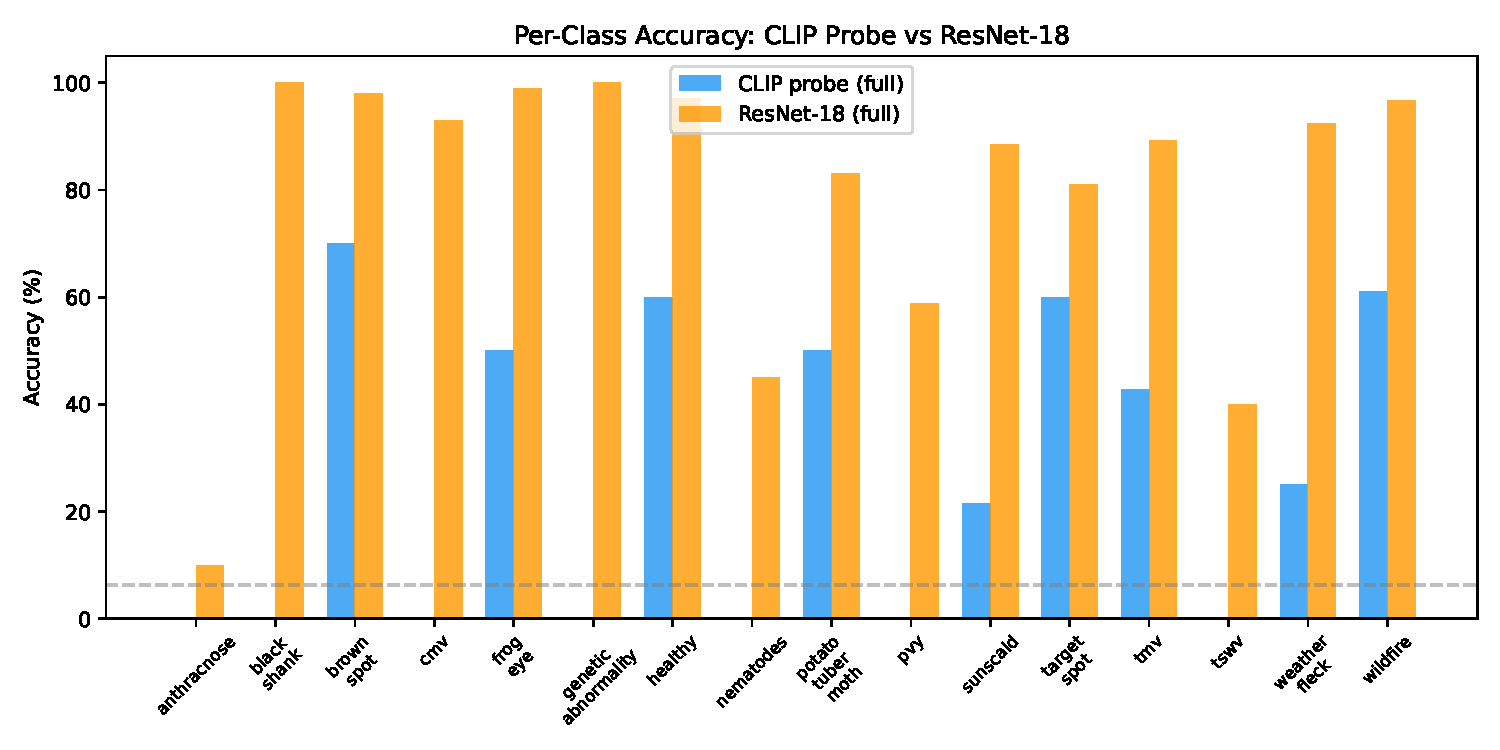
\includegraphics[width=\textwidth]{figures/fig_perclass.pdf}
 \caption{Per-class accuracy: full-data DFN-CLIP linear probe at the default $C{=}1$ (blue) vs.\ ResNet-18 (orange, representative seed). Note the CLIP curve uses the default $C{=}1$; the per-class values at the validation-selected $C{=}100$ are those of the \emph{CLIP best-$C$} column of Table~\ref{tab:perclass}. DFN-CLIP ($C{=}1$) reaches at least 50\% on 12 of 16 classes, while ResNet-18 reaches at least 50\% on 15 of 16. Dashed line: random chance (6.25\%). The blue/orange scheme is from the Okabe--Ito colorblind-safe palette.}
\label{fig:perclass}
\end{figure}

Per-class analysis (Figure~\ref{fig:perclass}, Table~\ref{tab:perclass}): CLIP reaches $\geq$50\% on 12/16 classes (default $C{=}1$); ResNet-18 on 15/16. CLIP is strongest on visually clean diseases, weakest on confusable ones (nematodes, PVY). Confusion matrices (Figure~\ref{fig:confusion}) show CLIP errors concentrated on a few overpredicted classes (brown\_spot, wildfire), while ResNet errors are more evenly spread.

\begin{figure}[!ht]
\centering
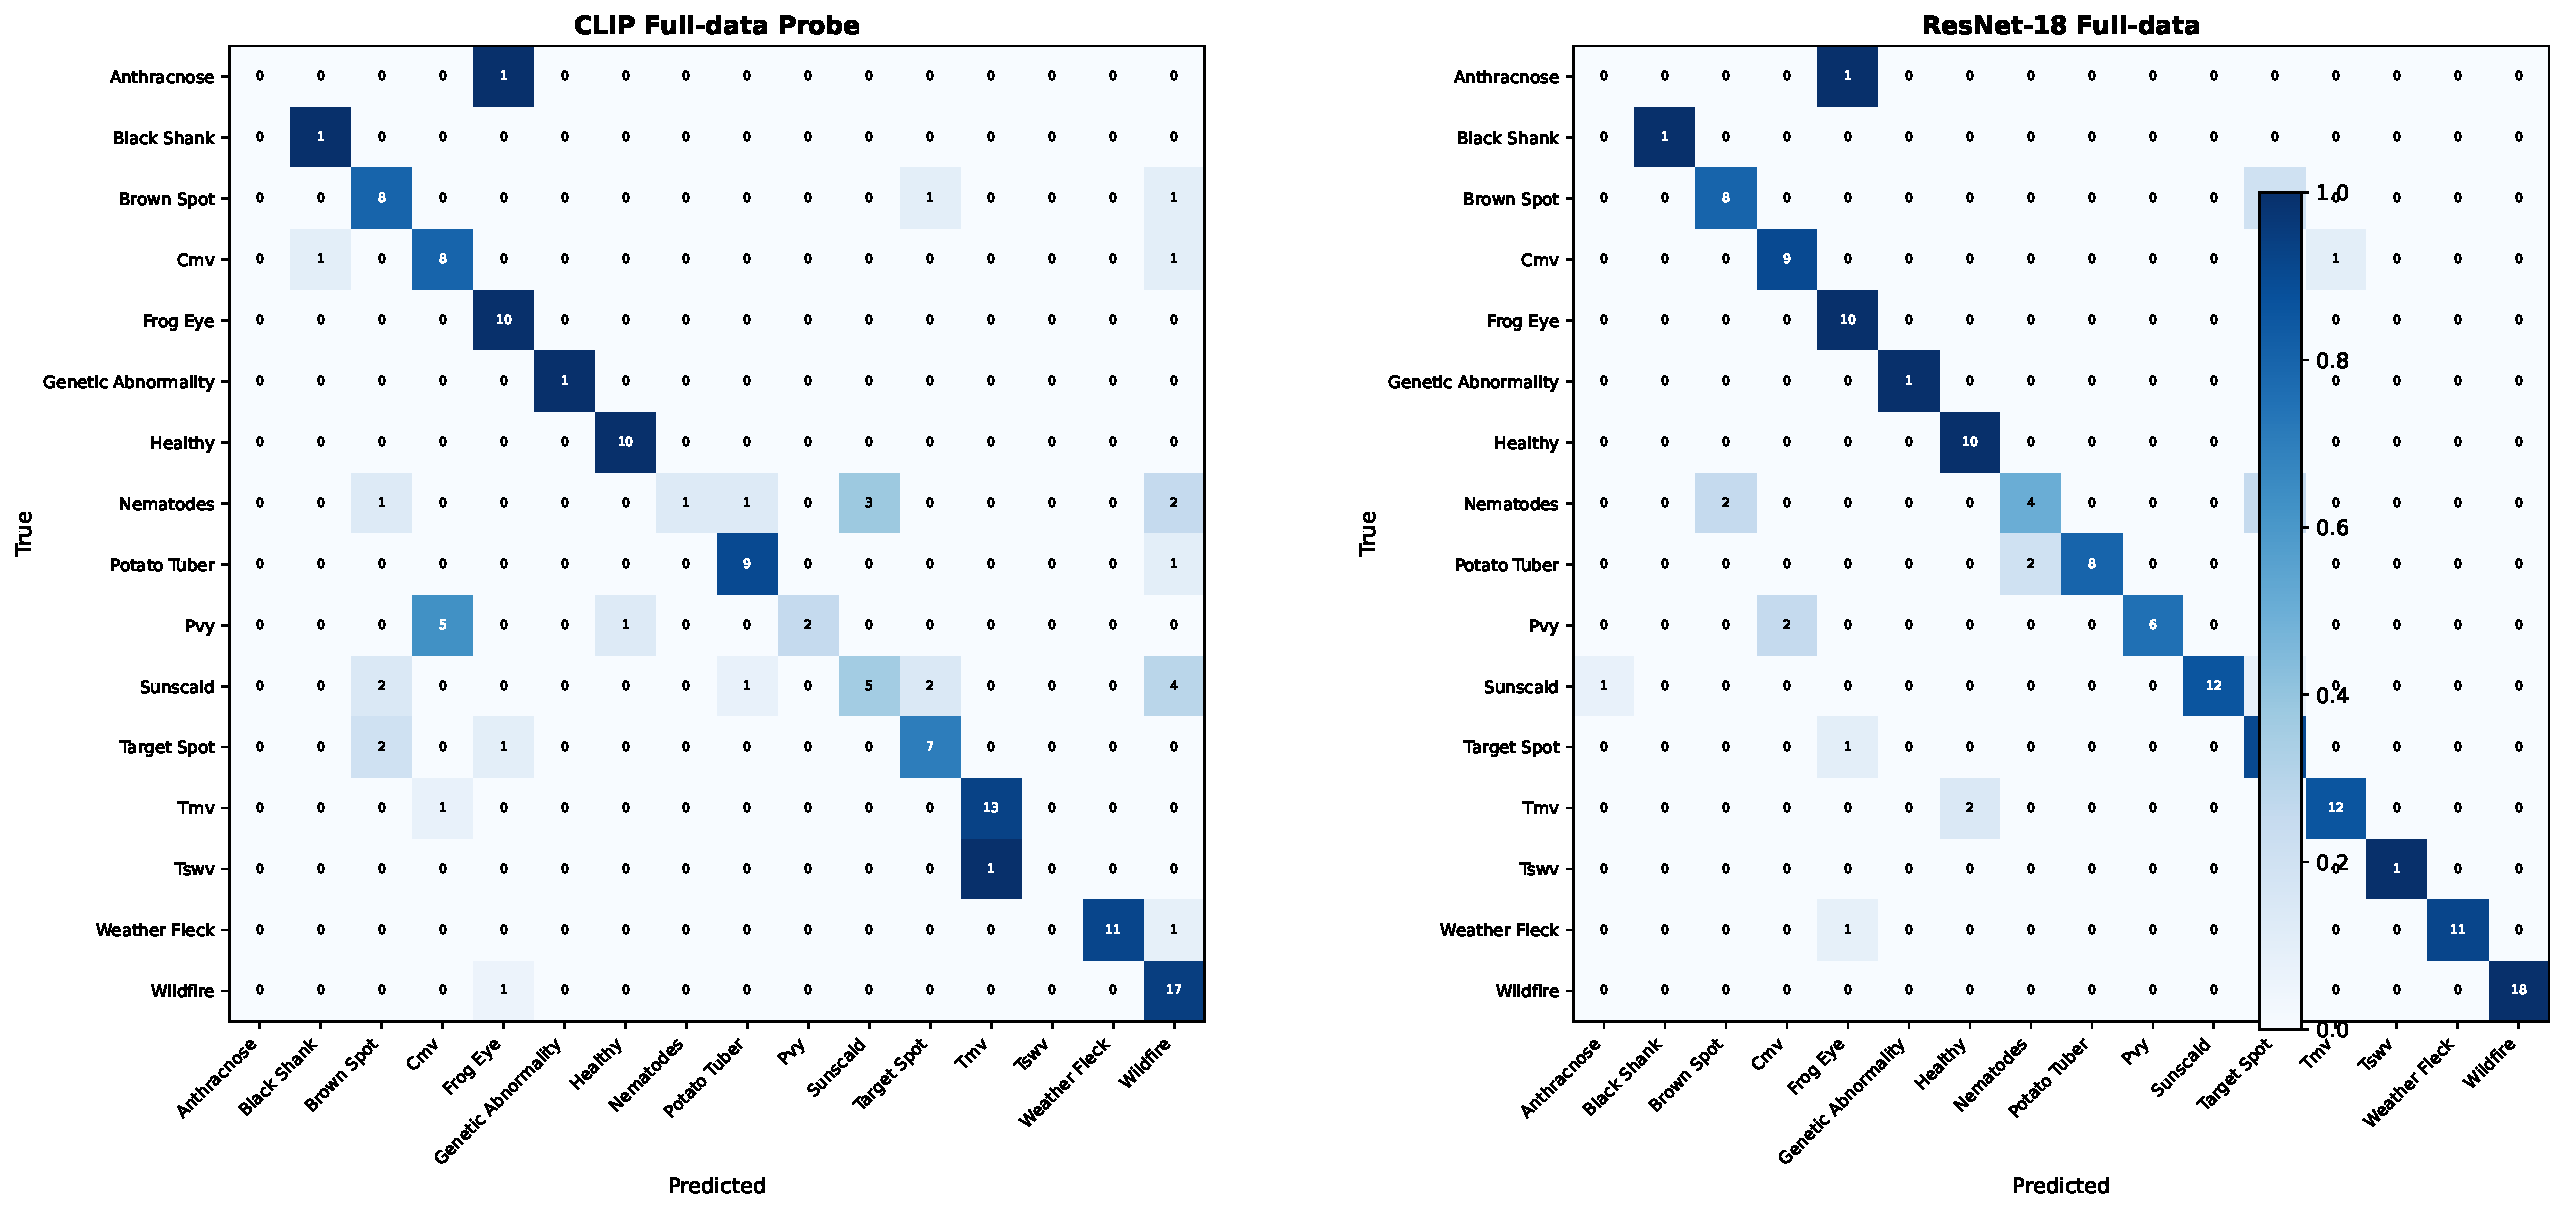
\includegraphics[width=\textwidth]{figures/fig_confusion.pdf}
\caption{Confusion matrices: CLIP probe ($C{=}1$, 76.8\%) vs.\ fine-tuned ResNet-18 (seed 0, 87.0\%; 15-seed mean 87.7\%$\pm$2.8\%). Row-normalised recall. Fine-tuned CLIP omitted (too few errors to show structure).}
\label{fig:confusion}
\end{figure}

\subsection{Why Does Generic CLIP Underperform on Fine-Grained Lesions?}
\label{sec:why}

\textbf{Feature geometry.} CLIP and frozen ResNet-18 features have broadly similar class-separation geometry: inter/intra ratio 0.81 (CLIP) vs.\ 0.79 (ResNet) on test; Fisher ratio 0.53 vs.\ 0.44; silhouette $\approx$0 for both. The CLIP--ResNet probe gap (76.8\% vs.\ 73.9\%) is therefore not explained by a large feature-geometry difference. $k$NN(1) on CLIP features reaches 71.7\%.

\textbf{Regularization, not representation.} Selecting $C$ on validation lifts the probe from 76.8\% to 86.2\% on the \emph{same} frozen features (Table~\ref{tab:cgrid}); the 256--64 MLP reaches only 85.5\% and $k$NN(1) 71.7\%. The frozen CLIP representation is not the binding constraint; the residual gap (1.5\,pp to fine-tuned ResNet) is within the test set's noise.

\textbf{Confusion structure.} Errors concentrate on visually confusable classes: nematodes$\to$sunscald (4/8), PVY$\to$CMV (4/8), target\_spot$\to$brown\_spot (2/10), weather\_fleck/sunscald$\to$wildfire (5/26). These depend on subtle lesion shape/texture/context rather than gross appearance.

\textbf{Checkpoint dependence.} The two checkpoints differ in pretraining corpus (DFN-CLIP applies a data-filtering network); the $K{=}1$ split (LAION within noise, DFN trailing $\approx$10\,pp) is plausibly related to corpus differences, but with only two checkpoints we cannot separate data, filtering, and recipe effects. CLIP's contrastive objective aligns holistic appearance with coarse labels, potentially privileging gross cues over the subtle local distinctions that separate the confusable classes.
\textbf{Readout geometry.} The classification load is checkpoint-dependent (Table~\ref{tab:readout}): on DFN-CLIP the CLS token carries essentially all signal (pure patch readouts 18.8--21.7\% vs.\ 76.8\% CLS at full data; best concatenation only $+2.2$\,pp), while on LAION-2B the patch tokens carry signal the CLS misses (mean-pool 87.0\% vs.\ 76.1\% CLS, $+10.9$\,pp). This is directionally consistent with weak-CLS-aggregation accounts~\cite{shi2026registers} and the medical small-lesion literature~\cite{cxr2026frozen,dinov3mil2026,traceclip2026}. We report this as a characterization, not a new method: the attention head we tested does not improve on the CLS probe on DFN-CLIP.

\begin{table}[!ht]
\centering
\caption{Checkpoint-dependent readout geometry on TPDD (138 test; image encoder frozen; logistic probe $C{=}1$; $K{=}5/10$ are 5-seed means, full data deterministic). \emph{mean-pool} is the pure patch-token readout; \emph{best $-$ CLS} is the largest gap over the full readout menu (mean-pool, max-pool, CLS$\oplus$mean, CLS$\oplus$max). The contrast is sharper than the \emph{best $-$ CLS} column alone shows: on DFN-CLIP every \emph{pure} patch-token readout is at or below the CLS token (mean-pool 18.8\%, max-pool 21.7\% at full data) and the only positive gap ($+2.2$\,pp) comes from a CLS$\oplus$max concatenation, whereas on LAION-2B even the pure mean-pool readout already exceeds the CLS token (87.0\% against 76.1\%). The DFN-CLIP full-data mean-pool value (18.8\%) is a $C{=}1$ underfitting artifact (the mean-pooled feature vector has a different scale that the default $C{=}1$ does not handle well), not a representational failure: at $K{=}10$ (5-seed), DFN-CLIP mean-pool reaches 47.0\% and CLS 55.7\%, consistent with the $K{<}10$ pattern.}
\label{tab:readout}
\begin{tabular}{llccc}
\toprule
\textbf{Checkpoint} & \textbf{$K$} & \textbf{CLS (\%)} & \textbf{mean-pool (\%)} & \textbf{best $-$ CLS} \\
\midrule
DFN-CLIP & full & 76.8 & 18.8 & $+2.2$\,pp \\
DFN-CLIP & 10 & 55.7 & 47.0 & $+0.6$\,pp \\
DFN-CLIP & 5 & 47.2 & 42.5 & $+2.5$\,pp \\
\midrule
LAION-2B & full & 76.1 & 87.0 & $+11.6$\,pp \\
LAION-2B & 10 & 66.4 & 70.7 & $+4.5$\,pp \\
LAION-2B & 5 & 59.7 & 65.4 & $+6.5$\,pp \\
\bottomrule
\end{tabular}
\end{table}

\textbf{Scale control.} ResNet-50 (25.6M, $\sim$2$\times$ ResNet-18) reaches 89.1\%$\pm$2.7 ($n{=}5$)---above ResNet-18 but below fine-tuned CLIP. The CNN--CLIP gap is not architecture-specific but the effects of scale, pretraining, and architecture cannot be separated on 1{,}295 images (\texttt{data/resnet50\_full.json}).

In summary: the frozen CLIP representation contains substantial disease-discriminative information (76--86\% with supervised heads) but it is not aligned with the zero-shot text-space decision geometry and is not optimally accessible to a default linear probe. The binding constraint is probe regularization, not representation quality.

%%%%%%%%%%%%%%%%%%%%%%%%%%%%%%%%%%%%%%%%%%
\section{Discussion}
\label{sec:discussion}

\subsection{Calibration Analysis}

Confidence is miscalibrated in both regimes. Zero-shot ECE is 0.05--0.06 but mean confidence is $\approx$1/16 (near-uniform), so the small ECE reflects near-constant confidence, not good calibration. The default $C{=}1$ probe has ECE 0.48 (systematically under-confident); selecting $C{=}100$ reduces this to 0.06, confirming the under-confidence is a regularization artifact. In neither regime are absolute confidence values calibrated for deployment without recalibration. With 138 test images, ECE bins are sparse; values should be read as directional (\texttt{data/calibration\_20261025.json}).

\subsection{Interpretation}

The core result is a protocol contrast, not a representational ranking. The frozen-probe comparison is conservative for CLIP: LoRA (0.19\% parameters) reaches 93.5\%, within 2.4\,pp of full fine-tuning, so compute is not the binding constraint. The frozen arm's value is practical (one-time feature cache, deterministic, isolates representation from adaptation), not accuracy-based. We do not convert it into a deployment recommendation; Section~\ref{sec:practical} states guidance on the axes where the two arms genuinely differ (iteration cost, inference cost) rather than on accuracy.

\subsection{Relation to Domain-Specific VLMs}

Our negative zero-shot result bounds \emph{off-the-shelf} CLIP only. SCOLD and BioCLIP~2 report zero-shot competence on fine-grained leaf tasks after domain-specific pretraining; we did not evaluate them beyond the single zero-shot control. The expected direction is that domain pretraining raises the zero-shot baseline, but the magnitude---and whether it closes the fine-grained gap---is an open question. LP++ (the one head-capacity control we did evaluate) improves the probe by up to $+14.7$\,pp few-shot, confirming that head capacity is a real but bounded source of gains that does not by itself lift zero-shot transfer.

\subsection{Knowledge-Graph Prompts}

KG-augmented prompts did not reliably outperform plain captions: on TPDD the best DFN-CLIP template is KG-Symptom (11.6\%) but below the 13.0\% baseline; on LAION-2B the three KG variants are mid-table (6.5--7.3\%). Two caveats: 7 of 16 TPDD classes lack KG descriptions (diluting any KG effect), and KG templates use tobacco-specific names that do not apply to TLD's 10-class vocabulary. No KG template for either checkpoint exceeds the majority-class baseline on either dataset.
It is therefore not claimed that knowledge-graph prompting is inherently ineffective; rather, the evaluated KG prompting strategy did not demonstrate a benefit under the present evaluation protocol and incomplete KG coverage.

\subsection{Deployment Cost Analysis}

A final, practice-oriented question underlies this section---given a compute budget, which model should a practitioner actually deploy? We answer it here rather than as a separate research question.

For deployment the decisive factor is inference cost rather than training cost, and the compact fine-tuned ResNet-18 is cheaper on both (Table~\ref{tab:cost}). Two scope limits apply to all deployment claims here: the accuracy evidence for the primary claims rests on controlled, close-up leaf imagery (TPDD, TLD); the field-condition evaluation (Section~\ref{sec:field}) provides directional but underpowered evidence for field generalization; and the cost figures in Table~\ref{tab:cost} are measurements on a desktop GPU (NVIDIA RTX 4070 Ti), not on actual edge hardware.
In a typical workflow both models are trained once (in the cloud or on a workstation) and then deployed for inference on lower-cost targets (mobile phones, field laptops, or on-tractor terminals); the comparison below is a relative one (ResNet-18 vs.\ CLIP), not an absolute certification for any particular device.
Under this framing, the relevant trade-offs are inference latency and memory, not training cost: on the measured desktop platform ResNet-18 is $\sim$34$\times$ faster at inference (3{,}900 vs.\ 116 images/s) and uses $\sim$3$\times$ less peak memory (1.1 vs.\ 3.5~GB), making it the more practical choice for resource-constrained inference if the desktop-GPU ordering carries over to edge hardware.
CLIP's advantage is confined to the classifier-training phase: once CLIP features have been extracted, the logistic-regression head can be trained on a CPU, which is useful for a quick research baseline (the feature-extraction step itself still requires the CLIP encoder).

\begin{table}[!ht]
\centering
\caption{Computational cost comparison (measured on NVIDIA RTX 4070 Ti, 12~GB; edge-hardware throughput not measured).}
\label{tab:cost}
\small
\begin{tabular}{lcc}
\toprule
\textbf{Factor} & \textbf{CLIP Probe} & \textbf{ResNet-18} \\
\midrule
Backbone training & No (frozen) & Yes (30 epochs) \\
Feature extraction & Yes (one-time, GPU) & Within training \\
Head training & Seconds (CPU) & Joint \\
Inference speed (batch 138, FP32) & $\sim$116 imgs/s & $\sim$3{,}900 imgs/s \\
Model size & 1.7 GB (428M params) & 11.6M params ($\sim$45 MB) \\
Peak memory (batch 138) & 3.5 GB & 1.1 GB \\
\midrule
Best accuracy (full, $C$ selected) & 86.2\% (DFN) / 87.7\% (LAION) & 87.7\% \\
\bottomrule
\end{tabular}
\smallskip
{\small Measured 2026-09-10 on a desktop GPU (NVIDIA RTX 4070 Ti, 12~GB); edge-hardware throughput was not measured. Inference throughput and peak memory at batch 138 (3 reps after 2 warmup); ResNet training time = mean of 15 full-data seeds (30 epochs). Exact values and protocol: \texttt{data/full\_provenance.json}.}
\end{table}

For deployment on lower-cost targets (mobile phones, field devices), ResNet-18 is the more practical choice on the measured desktop platform: it is $\sim$34$\times$ faster at inference and uses $\sim$3$\times$ less memory, though the desktop-GPU ordering has not been verified on edge hardware and the recommendation should be read as a relative, not a certified, comparison.
CLIP's training-phase advantage (the logistic head can be trained on a CPU once features are extracted) is relevant for a quick research baseline; for inference on resource-constrained devices the compact fine-tuned model is preferred.

\subsection{Practical Implications}
\label{sec:practical}

\begin{enumerate}
    \item \textbf{Do not rely on CLIP zero-shot for disease diagnosis.} No template exceeds the majority-class baseline on any dataset. Where misclassification is costly, route uncertain images to an expert.
    \item \textbf{Choose by the binding constraint; validate $C$ at small $K$.} If \emph{accuracy} governs: fine-tune CLIP or its LoRA adapter ($94.7$--$95.9\%$ full data, leads at every $K$). If \emph{inference cost} governs: deploy ResNet-18 ($\approx$34$\times$ faster, $\approx$3$\times$ less memory). If \emph{iteration speed} governs: use cached frozen features (bit-reproducible, head refit $<$1\,s). These are compatible, not contradictory. The default probe $C{=}1$ is under-regularized at small $K$ (the validation-selected $C$ improves it by up to $+10.1$\,pp at $K{=}2$ and $+9.4$--$11.6$\,pp at full data); validate $C$ on a held-out split at all $K$.
    \item \textbf{Treat CLIP confidence with care.} Zero-shot confidence is near-uniform; the default $C{=}1$ probe is under-confident (ECE 0.48). Recalibrate before deployment.
    \item \textbf{If using LAION-2B, check the readout geometry.} Mean-pooled patch readout reaches 87.0\% vs.\ 76.1\% CLS ($+10.9$\,pp) at $C{=}1$; the gain interacts with $C$ (CLS at $C{=}100$ reaches 87.7\%).
\end{enumerate}

\subsection{Limitations}

(1) Two CLIP checkpoints (both ViT-L/14) and one CNN family (ResNet/ConvNeXt) are tested; generalization to other architectures, crops, and domain-specific VLMs (SCOLD, BioCLIP~2) requires further study. SigLIP (878M) is competitive with CLIP on every axis, so the sigmoid objective does not change the qualitative picture.
(2) The CNN arm is not bit-reproducible at a fixed seed (cuDNN autotuning; three runs of seed 0 span 86.96--89.86\%). The 15-seed mean $\pm$ SD is the quantity to read; single-run CNN numbers carry a $\pm$1.5\,pp band.
(3) The full-data 1.5\,pp gap (86.2\% vs.\ 87.7\%) is within the test set's noise (95\% CI $[-0.1,+3.1]$\,pp); the 5-fold CV ($92.5\%$ vs.\ $89.4\%$, $p{=}0.002$) is the primary evidence. The fine-tuned-CLIP control is a restricted usage mode (image-label fine-tuning, not the full image--text objective); under CV the lead is $+1.2$\,pp (DFN, $p{=}0.12$) and $+2.3$\,pp (LAION, $p{=}0.03$), not the $+7$--$8$\,pp held-out gaps.
(4) Field results (53-image test, 19 classes) are directional, not statistically powered. The TLD dataset is community-contributed without a published protocol.
(5) The $C$-grid sweep is limited to $K{=}1/2$; the $K{=}5/10$ frozen-probe contrasts use default $C{=}1$ and could narrow under a $C$-matched comparison.
(6) The readout-geometry analysis uses one attention-head variant on the 138-image test split; the checkpoint-dependent CLS-vs-patch split is a directional observation, not a broad architectural finding.
(7) Analysis decisions were self-verified through independent re-runs but not independently re-derived by a second author; the code repository is provided for independent re-verification.


%%%%%%%%%%%%%%%%%%%%%%%%%%%%%%%%%%%%%%%%%%
\section{Conclusions}
\label{sec:conclusion}

We evaluated two generic CLIP checkpoints and a fine-tuned ResNet-18 across zero-shot, few-shot ($K{=}1/2/5/10$), and full-data regimes on tobacco (TPDD), with cross-crop checks on tomato and corn and a field-condition evaluation. The central finding is that the CLIP--ResNet ordering is determined by the adaptation protocol, not by the data regime: at the default $C{=}1$, the matched-budget ResNet leads or ties both CLIP probes at every $K$; with validation-selected $C$, LAION-2B reverses to a lead at $K{=}1/2$; under matched fine-tuning, CLIP leads at every $K$ for both checkpoints. At full data, the two are within 1.5\,pp on the held-out split (unresolvable) and ResNet holds a small, sign-stable edge under 5-fold CV ($92.5\%$ vs.\ $89.4\%$). Zero-shot CLIP shows no detectable improvement over the majority-class baseline on any dataset. Cross-crop checks confirm the protocol-dependent pattern; field conditions reverse the fine-tuned ranking (ResNet leads by 6.9\,pp), consistent with an image-style effect.

\textbf{Practical guidance:} (i) treat zero-shot CLIP as inadequate for fine-grained lesion diagnosis; (ii) fine-tune CLIP (or LoRA) where accuracy governs, deploy ResNet-18 where inference cost governs; (iii) the balanced-accuracy edge is a singleton-class artifact, not a deployable advantage; (iv) recalibrate confidence before deployment.

%%%%%%%%%%%%%%%%%%%%%%%%%%%%%%%%%%%%%%
\section*{Appendix A: Full-Data Protocol and Reproducibility}
\label{appx:protocol}

All full-data CLIP and frozen-ResNet numbers use a single deterministic feature-extraction protocol (clean transform, no augmentation; verified byte-identical across independent runs). The only stochastic side is the fine-tuned ResNet-18 ($n{=}15$ seeds). Row-by-row provenance for Table~\ref{tab:main}: frozen CLIP probes (deterministic, single fit); DINOv2 probe (deterministic); frozen ResNet-18 probe (deterministic); fine-tuned ResNet-18 ($n{=}15$ seeds); fine-tuned CLIP ($n{=}15$ seeds); LP++ and CoOp ($n{=}15$ seeds); LoRA ($n{=}15$ seeds); ConvNeXt-tiny ($n{=}15$ seeds); SigLIP probe (single run); SigLIP fine-tuned ($n{=}15$ seeds). Field dataset: 246 images, 19 classes; stratified split 193/53 (seed=0). Field class list: healthy (94), TMV (15), curl (15), bacterial wilt (11), downy mildew (11), red spot (10), black shank (10), anthracnose (9), blackleg (8), powdery mildew (8), damping-off (8), wildfire (7), angular leaf spot (7), black spot (7), frog-eye (6), sword-leaf (6), gray mold (5), leaf spot (5), herbicide damage (4).

\textbf{Feature-store unification.} Every canonical full-data number in the paper is computed on the single deterministic clean-transform store described above, and all full-data references have been reconciled onto that one store. A separate legacy store---built with the earlier stochastic training transform---drifts from it at the element level (maximum per-sample feature difference far above numerical noise), is flagged as such, and is never cited as canonical; where it is the internal reference of an adaptation control (the CoOp row), the drift is disclosed and scoped to that row's own comparisons rather than silently corrected. The only place the two stores move a headline value is the LAION-2B full-data probe: the legacy store gives 75.4\% where the canonical store gives 76.1\%, a 0.7\,pp store-level difference with no change of sign in any reported conclusion (LAION-2B still trails fine-tuned ResNet-18 at full data; against the matched-budget baseline the $K{=}1$ lead over the legacy baseline is a tie within noise). We report the canonical 76.1\% throughout and refer to this reconciliation onto one store as Feature-store unification.

\textbf{Row-by-row provenance of Table~\ref{tab:main}.} The ResNet-18 (fine-tuned) row mixes protocols: $K{=}1/2$ are legacy single-configuration runs, $K{=}5/10$ are matched-budget validation-selected means. LP++ and CoOp use the same canonical feature store; their per-$K$ probe references coincide with the canonical probe row at every $K$. CoOp's training stream of augmented views is intrinsic to its recipe and not used for evaluation.



%%%%%%%%%%%%%%%%%%%%%%%%%%%%%%%%%%%%%%%%%%
\section*{Author Contributions}
L.Z.\ and C.L.: conceptualization; L.Z.: methodology, software, formal analysis, investigation, data curation, writing--original draft, and visualization; L.Z.\ and F.H.: validation; C.L.\ and X.T.: resources and supervision; all authors: writing--review \& editing. L.Z.\ and C.L.\ are the corresponding authors.
\section*{Funding}
This research received no external funding.
\section*{Data Availability Statement}
The code, precomputed features, and per-seed result files supporting the findings of this study are available in an anonymized repository: \url{ANONYMOUS_REPOSITORY_URL_TO_BE_INSERTED_BEFORE_SUBMISSION}. The repository contains the full pipeline (feature extraction, probe and fine-tuning scripts, statistical analyses), the per-seed and per-fold result files cited as \texttt{data/*.json} throughout the text, and a manifest of the dataset splits; it is provided at the review stage so that the reported statistics can be independently re-verified.
\section*{Conflicts of Interest}
The authors declare no conflicts of interest.

\section*{Abbreviations}
The following abbreviations are used in this manuscript:
\par
\begin{tabular}{@{}l p{0.78\textwidth}@{}}
CLIP & Contrastive Language-Image Pretraining \\
ViT & Vision Transformer \\
TPDD & Tobacco Plant Disease Dataset \\
TLD & Tobacco Leaf Diseases dataset \\
KG & Knowledge Graph \\
CoOp & Context Optimization \\
ECE & Expected Calibration Error \\
PVY & Potato virus Y \\
CMV & Cucumber mosaic virus \\
TMV & Tobacco mosaic virus \\
TSWV & Tomato spotted wilt virus \\
CNN & Convolutional neural network \\
MLP & Multilayer perceptron \\
\end{tabular}

\vspace{6pt}

\begin{thebibliography}{99}

\bibitem{radford2021learning}
Radford, A.; Kim, J.W.; Hallacy, C.; Ramesh, A.; Goh, G.; Agarwal, S.; Sastry, G.; Askell, A.; Mishkin, P.; Clark, J.; et al.
Learning Transferable Visual Models From Natural Language Supervision.
In \emph{Proceedings of ICML}, 2021.
https://arxiv.org/abs/2103.00020

\bibitem{pdclip2026}
 Xie, P.; Li, X.; He, W.; Meadows, I.; Xiang, L.
 PD-CLIP: A contrastive language-image pre-training framework for zero-shot fine-grained plant disease diagnosis.
 \emph{Artif. Intell. Agric.} 2026.
 https://doi.org/10.1016/j.aiia.2026.08.012

\bibitem{huang2021gloria}
Huang, S.-C.; Shen, L.; Lungren, M.P.; Yeung, S.
GLoRIA: A Multimodal Global-Local Representation Learning Framework for Label-Efficient Medical Image Recognition.
In \emph{Proceedings of ICCV}, 2021.
https://doi.org/10.1109/iccv48922.2021.00391

\bibitem{liu2024remoteclip}
Liu, F.; Chen, D.; Guan, Z.; Zhou, X.; Zhu, J.; Ye, Q.; Fu, L.; Zhou, J.
RemoteCLIP: A Vision Language Foundation Model for Remote Sensing.
\emph{IEEE Trans. Geosci. Remote Sens.} 2024.
https://doi.org/10.1109/tgrs.2024.3390838

\bibitem{scold2025}
Nguyen, K.Q.; Le, L.T.T.; Quach, L.-D.
A Vision-Language Foundation Model for Leaf Disease Identification.
\emph{Expert Syst. Appl.} 2026.
https://doi.org/10.1016/j.eswa.2025.130084

\bibitem{bioclip2}
Gu, J.; Stevens, S.; Campolongo, E.; Thompson, M.; Zhang, N.; Wu, J.; Kopanev, A.; Mai, Z.; White, A.; Balhoff, J.; et al.
BioCLIP 2: Emergent Properties from Scaling Hierarchical Contrastive Learning.
In \emph{Advances in Neural Information Processing Systems (NeurIPS)}, 2025.
https://doi.org/10.52202/085713-3436

\bibitem{lpplus}
Huang, Y.; Shakeri, F.; Dolz, J.; Boudiaf, M.; Bahig, H.; Ben Ayed, I.
LP++: A Surprisingly Strong Linear Probe for Few-Shot CLIP.
In \emph{Proceedings of CVPR}, 2024.
https://doi.org/10.1109/cvpr52733.2024.02244

\bibitem{shi2026registers}
Shi, C.; Yu, Y.; Yang, S.
Vision Transformers Need More Than Registers.
\emph{arXiv preprint} arXiv:2602.22394, 2026; accepted to CVPR 2026.
https://doi.org/10.48550/arXiv.2602.22394

\bibitem{cxr2026frozen}
Muthyala, R.; Yin, Z.; Jilla, A.; Li, F.; Dapamede, T.; Khosravi, B.; Chavoshi, M.; Gichoya, J.~W.; Purkayastha, S.
Frozen Foundation-Model Embeddings Discard Small-Lesion Signal in Chest Radiography: Implications for Pre-Deployment Evaluation.
\emph{arXiv preprint} arXiv:2606.11606, 2026.
https://doi.org/10.48550/arXiv.2606.11606

\bibitem{traceclip2026}
Liu, X.; Shi, S.; Chen, Y.; Wang, G.; Yao, X.-W.; Zhong, S.
TraceCLIP: Recovering Local Semantics from Patch-to-CLS Contributions.
\emph{arXiv preprint} arXiv:2607.26107, 2026.
https://doi.org/10.48550/arXiv.2607.26107

\bibitem{dinov3mil2026}
Pramod Kumar, P.; Vishalakshi, M.; Sharma, S.
DINOv3-MIL: Per-Kidney Multi-Label Tumour and Cyst Detection from Foundation-Model Patch Tokens on KiTS23.
\emph{arXiv preprint} arXiv:2607.22687, 2026.
https://doi.org/10.48550/arXiv.2607.22687

\bibitem{zhai2023sigmoid}
Zhai, X.; Mustafa, B.; Kolesnikov, A.; Beyer, L.
Sigmoid Loss for Language Image Pre-Training.
In \emph{Proceedings of ICCV}, 2023.
https://doi.org/10.1109/iccv51070.2023.01100

\bibitem{cherti2023reproducible}
Cherti, M.; Beaumont, R.; Wightman, R.; Wortsman, M.; Ilharco, G.; Gordon, C.; Schuhmann, C.; Schmidt, L.; Jitsev, J.
Reproducible Scaling Laws for Contrastive Language-Image Learning.
In \emph{Proceedings of CVPR}, 2023.
https://doi.org/10.1109/cvpr52729.2023.00276

\bibitem{ilharco2022openclip}
Ilharco, G.; Wortsman, M.; Carlini, N.; Taori, R.; Dave, A.; Shankar, V.; Namkoong, H.; Miller, J.; Hajishirzi, H.; Farhadi, A.; Schmidt, L.
OpenCLIP.
\emph{Zenodo Software}, 2021.
Available online: \url{https://doi.org/10.5281/zenodo.5143773}.

\bibitem{deng2009imagenet}
Deng, J.; Dong, W.; Socher, R.; Li, L.-J.; Li, K.; Fei-Fei, L.
ImageNet: A Large-Scale Hierarchical Image Database.
In \emph{Proceedings of CVPR}, 2009.
https://doi.org/10.1109/cvpr.2009.5206848

\bibitem{stevens2024bioclip}
Stevens, S.; Wu, J.; Thompson, M.J.; Campolongo, E.G.; Song, C.H.; Carlyn, D.E.; Dong, L.; Dahdul, W.M.; Stewart, C.; Berger-Wolf, T.; et al.
BioCLIP: A Vision Foundation Model for the Tree of Life.
In \emph{Proceedings of CVPR}, 2024.
https://doi.org/10.1109/cvpr52733.2024.01836

\bibitem{shinoda2025agrobench}
Shinoda, R.; Inoue, N.; Kataoka, H.; Onishi, M.; Ushiku, Y.
AgroBench: Vision-Language Model Benchmark in Agriculture.
In \emph{Proceedings of ICCV}, 2025, 7634--7644.
https://doi.org/10.1109/iccv51701.2025.00716

\bibitem{zhou2022learning}
Zhou, K.; Yang, J.; Loy, C.C.; Liu, Z.
Learning to Prompt for Vision-Language Models.
\emph{Int. J. Comput. Vis.} 2022, 130, 2337--2348.
https://doi.org/10.1007/s11263-022-01653-1

\bibitem{liu2025finegrained}
Liu, Y.; Deng, Y.; Liu, A.; Liu, Y.; Li, S.
Fine-Grained Multi-Modal Prompt Learning for Vision-Language Models.
\emph{Neurocomputing} 2025, 636, 130028.
https://doi.org/10.1016/j.neucom.2025.130028

\bibitem{cropdpkg2025}
Yan, R.; An, P.; Meng, X.; Li, Y.; Li, D.; Xu, F.; Dang, D.
A Knowledge Graph for Crop Diseases and Pests in China.
\emph{Scientific Data} 2025, 12, 222.
https://doi.org/10.1038/s41597-025-04492-0

\bibitem{argueso2020fewshot}
Argüeso, D.; Picon, A.; Irusta, U.; Medela, A.; San-Emeterio, M.G.; Bereciartua, A.; Alvarez-Gila, A.
Few-Shot Learning Approach for Plant Disease Classification Using Images Taken in the Field.
\emph{Computers and Electronics in Agriculture} 2020, 175, 105542.
https://doi.org/10.1016/j.compag.2020.105542

\bibitem{liang2021cotton}
Liang, X.
Few-Shot Cotton Leaf Spots Disease Classification Based on Metric Learning.
\emph{Plant Methods} 2021, 17, 114.
https://doi.org/10.1186/s13007-021-00813-7

\bibitem{plantvillage2016}
Mohanty, S.P.; Hughes, D.P.; Salathé, D.
Using Deep Learning for Image-Based Plant Disease Detection.
\emph{Front. Plant Sci.} 2016, 7, 1419.
https://doi.org/10.3389/fpls.2016.01419

\bibitem{lin2022tpdd}
Lin, H.; Tse, R.; Tang, S.-K.; Qiang, Z.; Ou, J.; Pau, G.
Tobacco Plant Disease Dataset.
In \emph{Proceedings of the 14th International Conference on Digital Image Processing (ICDIP)}, 2022, 89.
https://doi.org/10.1117/12.2644288

\bibitem{lin2024tla}
Lin, H.; Qiang, Z.; Tse, R.; Tang, S.-K.; Pau, G.
A Few-Shot Learning Method for Tobacco Abnormality Identification.
\emph{Front. Plant Sci.} 2024, 15, 1333236.
https://doi.org/10.3389/fpls.2024.1333236

\bibitem{tld}
Joker5800.
Tobacco\_Leaf\_Diseases.
\emph{Hugging Face Datasets}, 2024.
Available online: \url{https://huggingface.co/datasets/Joker5800/Tobacco_Leaf_Diseases}.

\bibitem{plantvillage_mendeley}
Data for: Identification of Plant Leaf Diseases Using a 9-layer Deep Convolutional Neural Network.
\emph{Mendeley Data}, 2019.
https://doi.org/10.17632/tywbtsjrjv.1

\bibitem{fang2023data}
Fang, A.; Jose, A.M.; Jain, A.; Schmidt, L.; Toshev, A.; Shankar, V.
Data Filtering Networks.
\emph{arXiv preprint} arXiv:2309.17425, 2023.

\bibitem{he2016deep}
He, K.; Zhang, X.; Ren, S.; Sun, J.
Deep Residual Learning for Image Recognition.
In \emph{Proceedings of CVPR}, 2016.
https://doi.org/10.1109/cvpr.2016.90

\bibitem{dinov2}
Oquab, M.; Darcet, T.; Moutakanni, T.; et al.
DINOv2: Learning Robust Visual Features without Supervision.
\emph{Transactions on Machine Learning Research (TMLR)}, 2024.
https://arxiv.org/abs/2304.07193

\bibitem{hu2022lora}
Hu, E.~J.; Shen, Y.; Wallis, P.; et al.
LoRA: Low-Rank Adaptation of Large Language Models.
In \emph{Proceedings of ICLR}, 2022.
https://arxiv.org/abs/2106.09685

\bibitem{liu2022convnext}
Liu, Z.; Mao, H.; Wu, C.-Y.; Feichtenhofer, C.; Darrell, T.; Xie, S.
A ConvNet for the 2020s.
In \emph{Proceedings of CVPR}, 2022.
https://arxiv.org/abs/2201.03545

\end{thebibliography}

%%%%%%%%%%%%%%%%%%%%%%%%%%%%%%%%%%%%%%%%%%
\section*{Appendix: Supplementary Figure}

\begin{figure}[!ht]
\centering
\includegraphics[width=0.85\textwidth]{figures/fig_feature_space.pdf}
\caption{t-SNE projection of frozen CLIP features on the 138-image TPDD test set (perplexity=30, max\_iter=1000, random\_state=42). The visually confusable nematodes/PVY/CMV/sunscald group shares feature space; the projection is consistent with the quantitative inter/intra-class geometry reported in the main text but, on 138 points, is not stable across perplexity or seed choices and is included only as an illustrative view, not as evidence.}
\label{fig:tsne}
\end{figure}

\end{document}
